\documentclass[aspectratio=169,t]{beamer}

\usetheme{XDC}
\usepackage[utf8]{inputenc}

\author{Friedrich Vock}

\title{Improving the World's Slowest Raytracer}

\date{October 17, 2023}

\setBackground{graphics/frogrender.png}

\chapterIntroConfig

\begin{document}

\begin{slide}
\titlepage
\end{slide}

\defaultConfig

\begin{slide}{Contents}
\tableofcontents
\end{slide}

\section{Raytracing: A Quick Recap}

\chapterIntroConfig
\begin{slide}{Raytracing: A Quick Recap}
\end{slide}
\defaultConfig

\subsection{Acceleration Structures}
\begin{slide}{Acceleration Structures}
    \begin{itemize}
     \item Opaque from the app's POV
     \item Contains scene geometry in format understood by ray accelerator HW
     \item Built by the driver, app provides ``primitive soup''
     \item Three primitive types: Triangles, AABBs and instances of other BVHs
     \begin{itemize}
      \item With AABB primitives, a shader can execute custom code to determine if a ray hits the surface
      \item Vulkan defines two levels of acceleration structures: Top-Level and Bottom-Level
      \begin{itemize}
        \item TLAS can only have BLAS instances as primitives
        \item BLAS can only have triangles or AABBs as primitives
      \end{itemize}
     \end{itemize}
    \end{itemize}
\end{slide}
\subsection{Raytracing Pipelines}

\begin{slide}{Raytracing Pipelines}
    \begin{itemize}
     \item Special type of pipeline for performing raytracing
     \item New shader stages: Ray Generation, Any Hit, Intersection, Closest Hit, Miss, Callable
    \end{itemize}
    \pause
    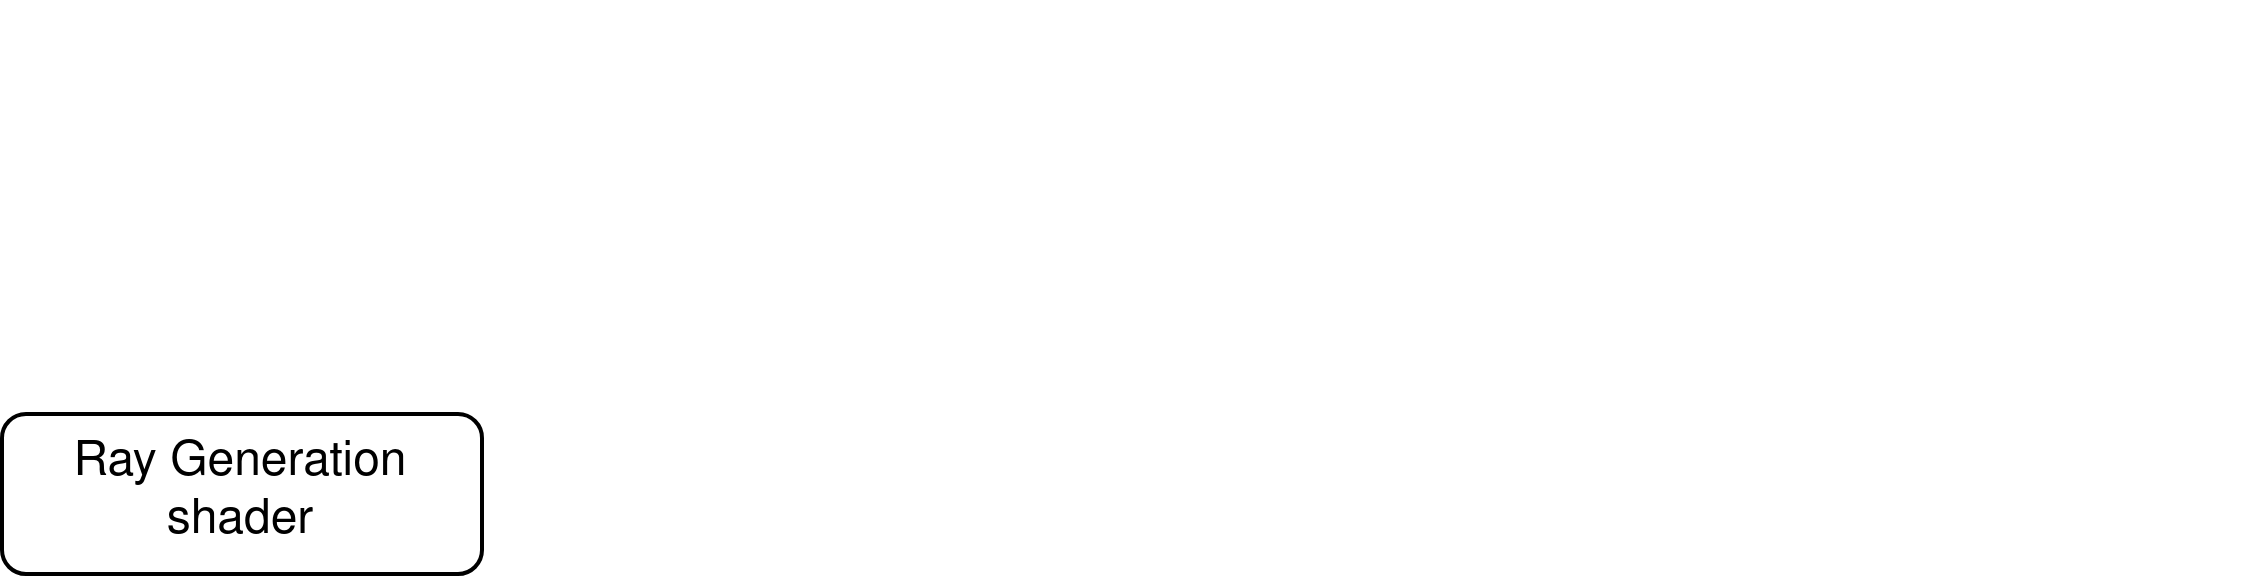
\includegraphics[width=0.95\linewidth]{graphics/RTStages1.png}
\end{slide}

\begin{slide}{Raytracing Pipelines}
    \begin{itemize}
     \item Special type of pipeline for performing raytracing
     \item New shader stages: Ray Generation, Any Hit, Intersection, Closest Hit, Miss, Callable
    \end{itemize}
    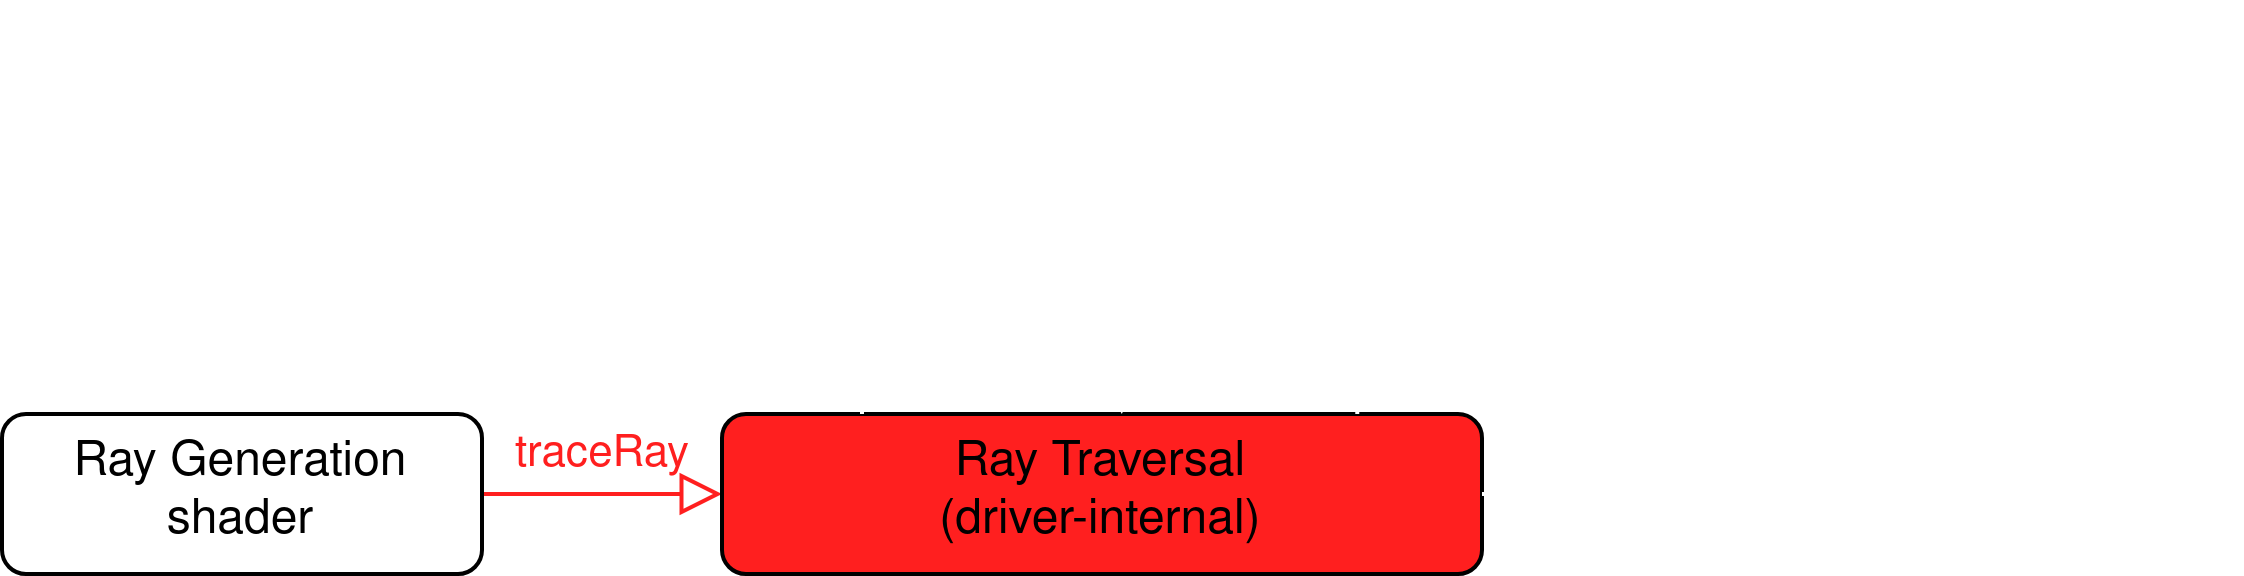
\includegraphics[width=0.95\linewidth]{graphics/RTStages2.png}
\end{slide}

\begin{slide}{Raytracing Pipelines}
    \begin{itemize}
     \item Special type of pipeline for performing raytracing
     \item New shader stages: Ray Generation, Any Hit, Intersection, Closest Hit, Miss, Callable
    \end{itemize}
    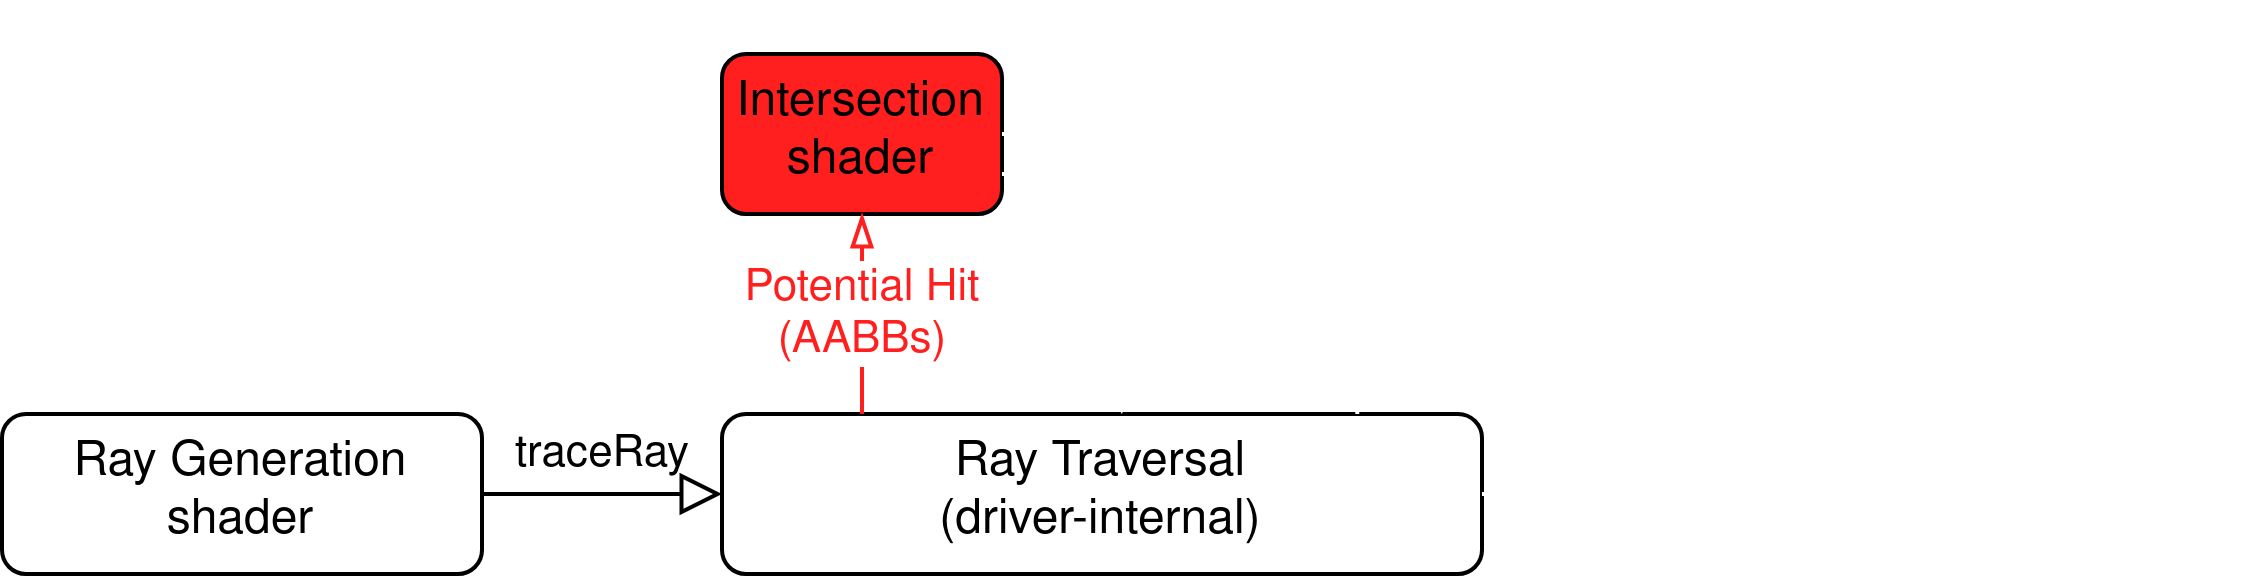
\includegraphics[width=0.95\linewidth]{graphics/RTStages3.png}
\end{slide}

\begin{slide}{Raytracing Pipelines}
    \begin{itemize}
     \item Special type of pipeline for performing raytracing
     \item New shader stages: Ray Generation, Any Hit, Intersection, Closest Hit, Miss, Callable
    \end{itemize}
    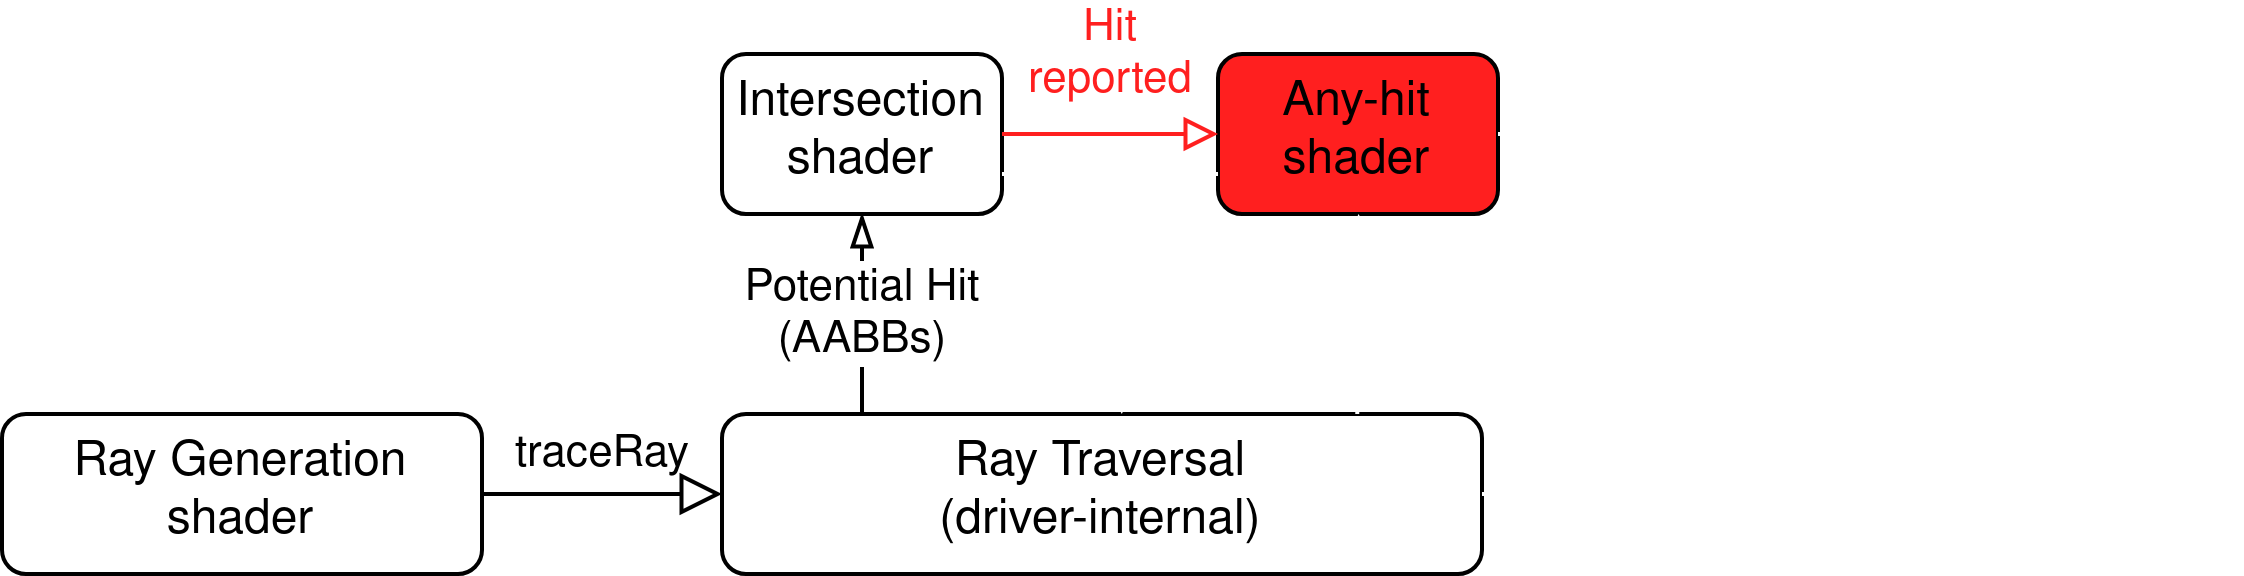
\includegraphics[width=0.95\linewidth]{graphics/RTStages4.png}
\end{slide}

\begin{slide}{Raytracing Pipelines}
    \begin{itemize}
     \item Special type of pipeline for performing raytracing
     \item New shader stages: Ray Generation, Any Hit, Intersection, Closest Hit, Miss, Callable
    \end{itemize}
    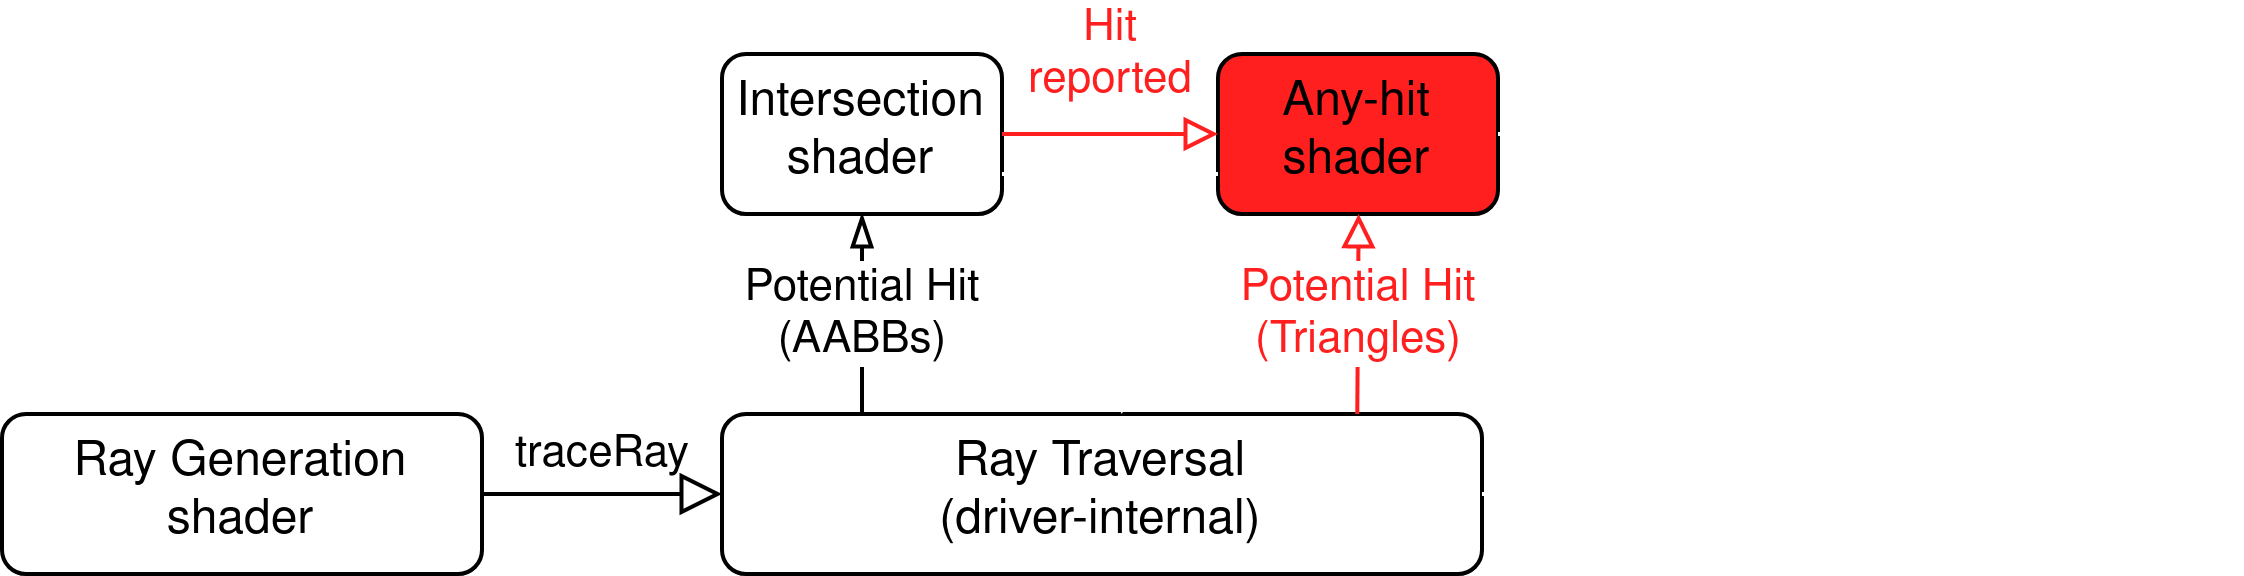
\includegraphics[width=0.95\linewidth]{graphics/RTStages5.png}
\end{slide}

\begin{slide}{Raytracing Pipelines}
    \begin{itemize}
     \item Special type of pipeline for performing raytracing
     \item New shader stages: Ray Generation, Any Hit, Intersection, Closest Hit, Miss, Callable
    \end{itemize}
    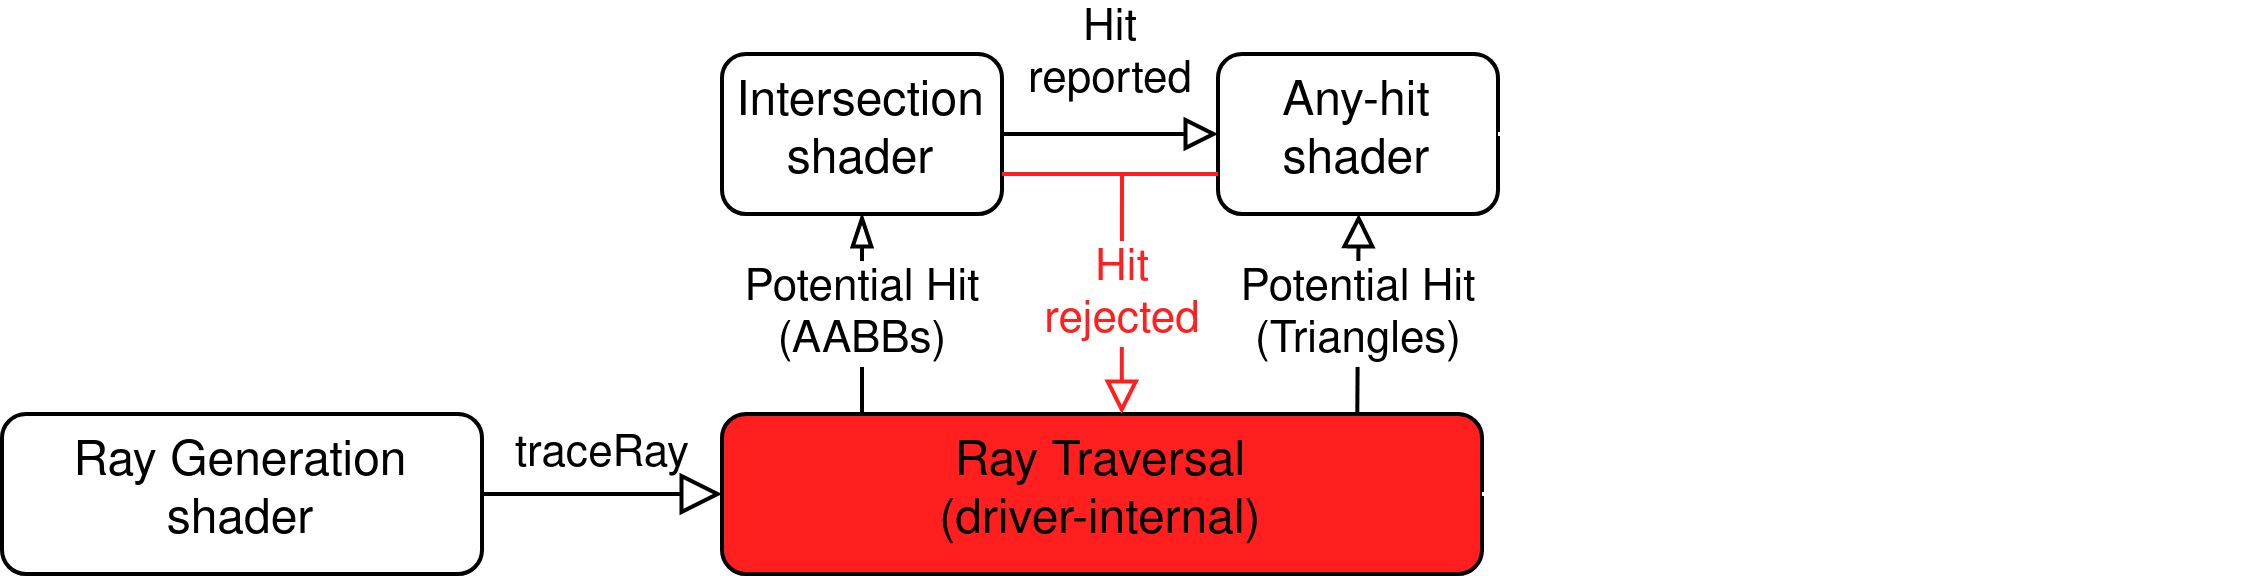
\includegraphics[width=0.95\linewidth]{graphics/RTStages6.png}
\end{slide}

\begin{slide}{Raytracing Pipelines}
    \begin{itemize}
     \item Special type of pipeline for performing raytracing
     \item New shader stages: Ray Generation, Any Hit, Intersection, Closest Hit, Miss, Callable
    \end{itemize}
    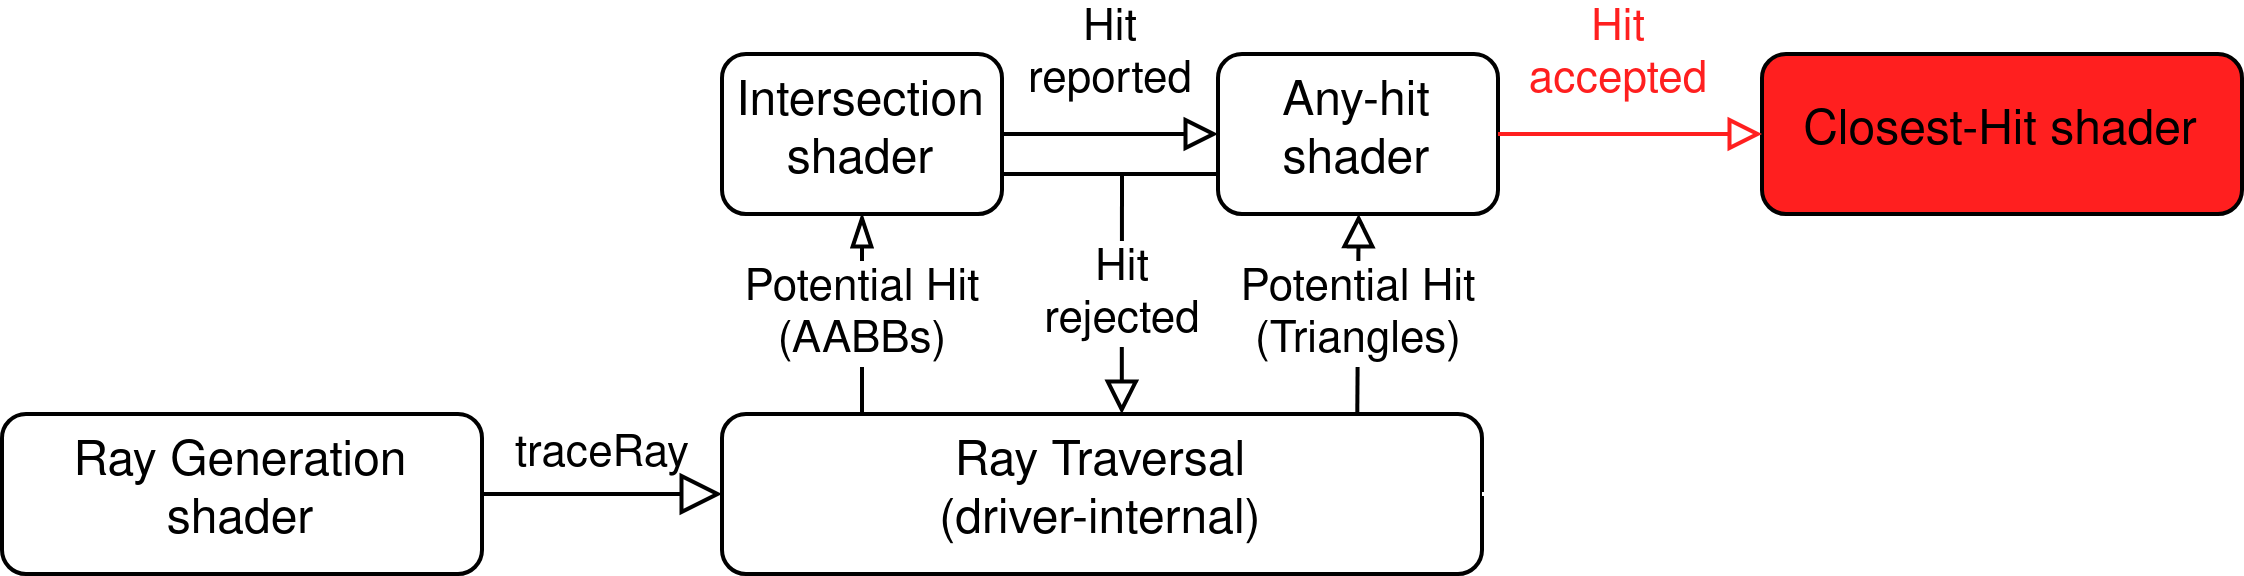
\includegraphics[width=0.95\linewidth]{graphics/RTStages7.png}
\end{slide}

\begin{slide}{Raytracing Pipelines}
    \begin{itemize}
     \item Special type of pipeline for performing raytracing
     \item New shader stages: Ray Generation, Any Hit, Intersection, Closest Hit, Miss, Callable
    \end{itemize}
    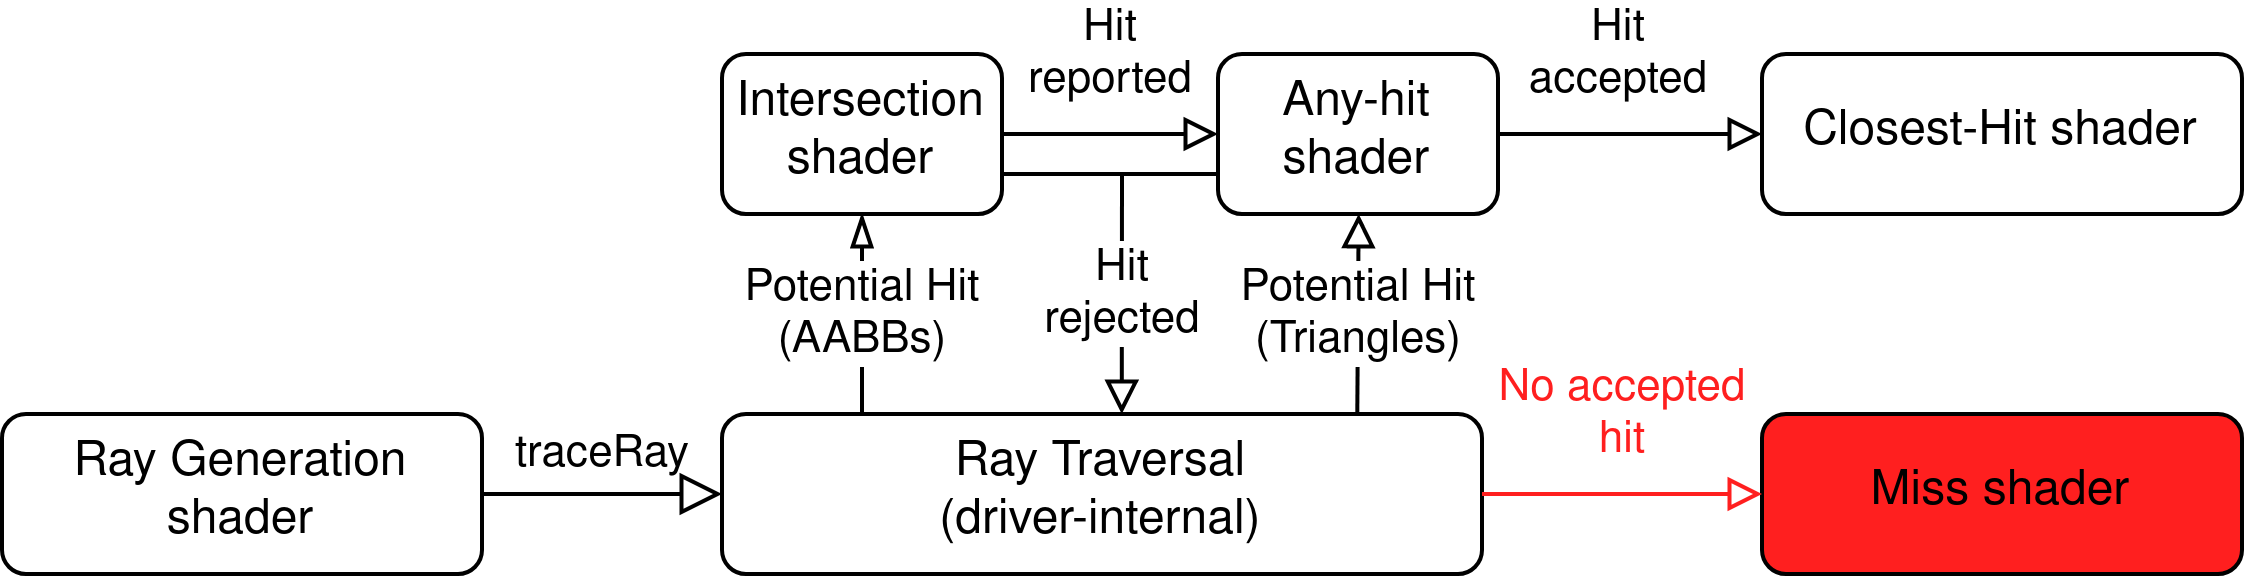
\includegraphics[width=0.95\linewidth]{graphics/RTStages8.png}
\end{slide}

\begin{slide}{Raytracing Pipelines}
    \begin{itemize}
     \item Special type of pipeline for performing raytracing
     \item New shader stages: Ray Generation, Any Hit, Intersection, Closest Hit, Miss, Callable
    \end{itemize}
    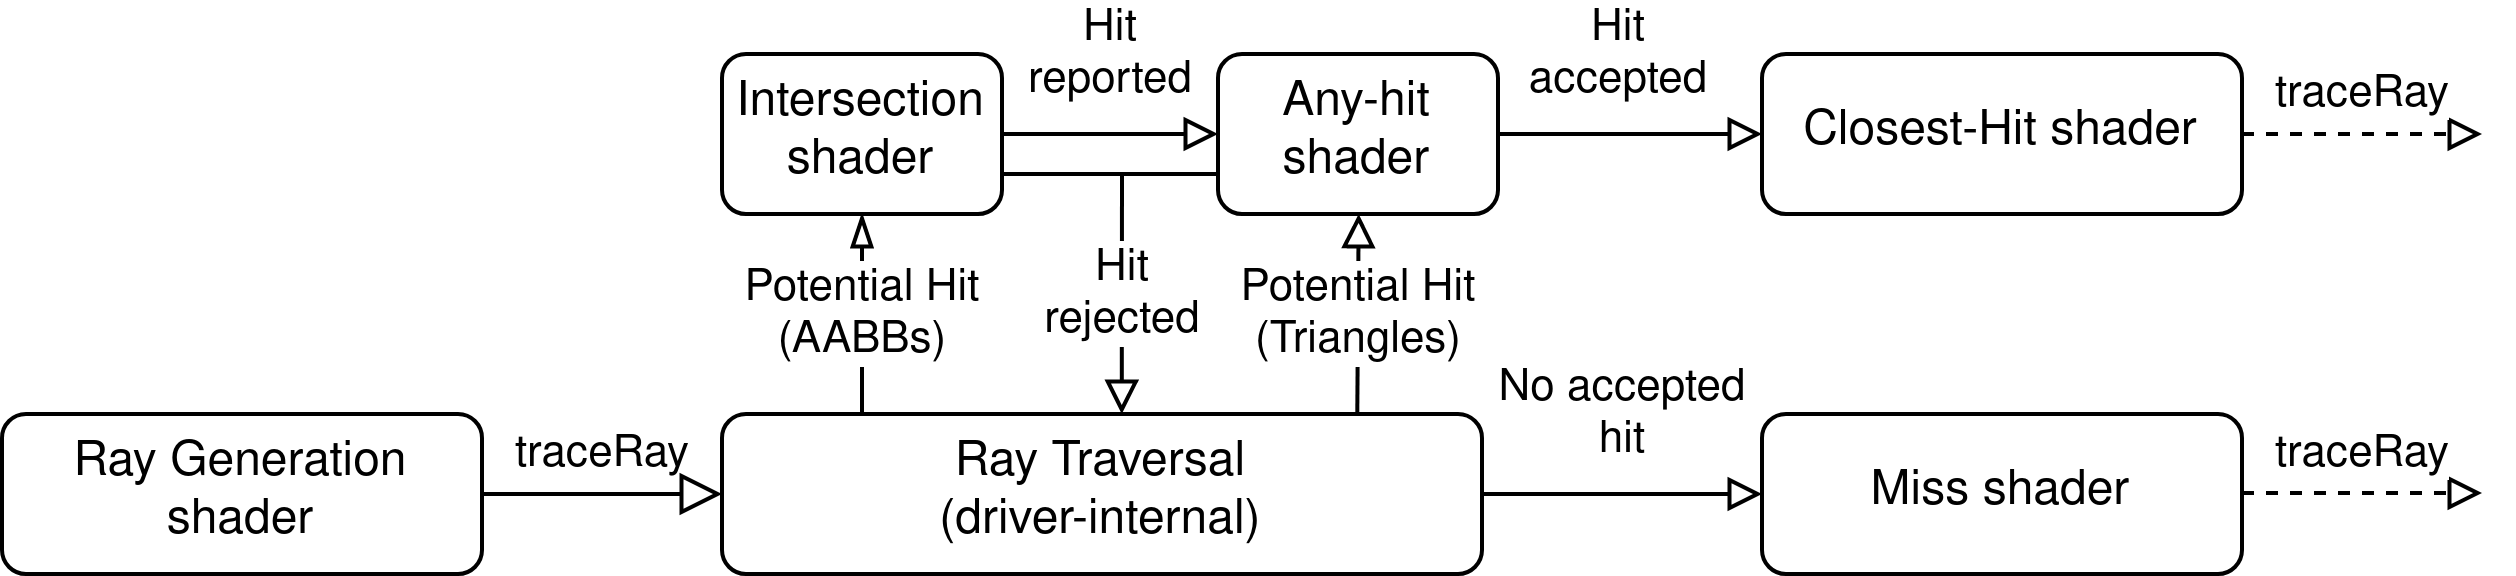
\includegraphics[width=1.0651\linewidth]{./graphics/RTStages9.png}
    \pause
    \begin{itemize}
    \item Callable shaders can be called from any stage
    \end{itemize}
\end{slide}

\begin{slide}{Other RT Pipeline concepts}
    \begin{itemize}
      \item Shader Binding Tables (SBTs)
      \begin{itemize}
       \item More than one shader for each stage!
       \item App tells the driver which shader to call with a Shader Binding Table
       \item Jump Table on the GPU
      \end{itemize}
      \item Pipeline Libraries
      \begin{itemize}
       \item Incomplete pipelines that can be linked with other pipelines
       \item Useful for e.g. moving commonly-used shaders into common library
      \begin{itemize}
       \item Pipelines using these shaders only need to link to the previously-created library
      \end{itemize}
      \end{itemize}

    \end{itemize}
\end{slide}

\section{Implementing Acceleration Structures}

\chapterIntroConfig
\begin{slide}{Implementing Acceleration Structures}
\end{slide}
\defaultConfig

\begin{slide}{Acceleration Structure Building}
 \begin{itemize}
  \item RADV implements acceleration structures as BVHs
  \begin{itemize}
    \item Tree of AABBs and triangles
    \item Internal nodes are AABBs, leaf nodes are AABB/triangle/BLAS pointer
    \item A node's AABB is the AABB of its child nodes
  \end{itemize}
  \item Hardware format is BVH4
  \begin{itemize}
    \item Each internal node can have up to 4 child nodes
  \end{itemize}
 \end{itemize}

 \begin{minipage}[t]{0.45\textwidth}
% now that's a way to write code
\texttt{struct radv\_bvh\_box32\_node \{\\
\hspace*{8pt} uint32\_t children[4];\\
\hspace*{8pt} radv\_aabb coords[4];\\
\hspace*{8pt} uint32\_t reserved[4];\\
\};}
 \end{minipage}
 \begin{minipage}[t]{0.5\textwidth}
\texttt{struct radv\_bvh\_triangle\_node \{}\\
\texttt{\hspace*{8pt} float coords[3][3];}\\
\texttt{\hspace*{8pt} uint32\_t reserved[3];}\\
\texttt{\hspace*{8pt} uint32\_t triangle\_id;}\\
\texttt{\hspace*{8pt} /* flags in upper 4 bits */}\\
\texttt{\hspace*{8pt} uint32\_t geometry\_id\_and\_flags;}\\
\texttt{\hspace*{8pt} uint32\_t reserved2;}\\
\texttt{\hspace*{8pt} uint32\_t id;}\\
\texttt{\};}
 \end{minipage}
\end{slide}


\begin{slide}{Acceleration Structure Building}
 \begin{itemize}
  \item Building acceleration structures is a multi-step process
  \begin{enumerate}
   \item Convert input primitives to leaf nodes
   \item Sort nodes
   \item Construct binary BVH
   \item Convert binary BVH to BVH4
  \end{enumerate}
  \item Need barriers in between each step!
  \begin{itemize}
   \item Bad for building many tiny acceleration structures
   \item Vulkan allows for building multiple acceleration structures at a time
  \end{itemize}
 \end{itemize}
\end{slide}

\begin{slide}{Acceleration Structure Building}
  \begin{itemize}
   \item
  \end{itemize}
\end{slide}

\subsection{LBVH}

\begin{slide}{Linear BVH}
  \begin{itemize}
   \item Algorithm from 2014
   \item Builds a radix tree from generated morton codes
   \item Tree can be built up independently for each node
   \begin{itemize}
    \item Great for parallelization!
   \end{itemize}
   \item Used for quick builds
  \end{itemize}
\end{slide}

\subsection{PLOC}

\begin{slide}{Parallel Locally-Ordered Clustering}
  \begin{itemize}
   \item Algorithm from 2017
   \item Better quality than LBVH, though slower
   \item Original reference implementation was written in CUDA
   \item Heavily relies on device-wide synchronization
   \begin{itemize}
    \item No global synchronization primitives available
    \item Have to make our own!
   \end{itemize}
  \end{itemize}
\end{slide}

\begin{slide}{The Poor Man's Global Synchronization}
  \begin{itemize}
   \item All build shaders are written in Vulkan GLSL
   \item Compiler and target hardware is known
   \item Can assume more guarantees in certain aspects
   \begin{itemize}
    \item Forward Progress
    \item Launch ordering
   \end{itemize}
   \item Work Stealing Queue
   \begin{itemize}
    \item Each task receives a unique ID
    \item Runtime-defined number of tasks to launch before synchronizing
   \end{itemize}
   Launching new tasks:\\
   \pause
   \texttt{taskID = atomicAdd(taskStartedCounter, 1);}\\
  \end{itemize}
\end{slide}

\begin{slide}{The Poor Man's Global Synchronization}
   Making sure previous work has finished:\\
  \begin{itemize}
   \item Maintain a ``tasks finished'' counter and increment it when finished
   \item If the new work ID is larger than the maximum task ID to launch before synchronizing, busy-wait until the maximum task ID is updated
   \item The last task to finish updates the maximum task ID
  \end{itemize}

  \texttt{finishID = atomicAdd(taskFinishCounter, 1);\\
  if (finishID == maxTaskID) \{\\
  \hspace*{8pt}atomicAdd(maxTaskID, nextNumberOfTasks);\\
  \}
  else \{\\
  \hspace*{8pt}while (taskID > maxTaskID) \{\}\\
  \}
  }\\
\end{slide}

\section{Implementing Raytracing Pipelines}

\chapterIntroConfig
\begin{slide}{Implementing Raytracing Pipelines}
\end{slide}
\defaultConfig

\begin{slide}{Hardware Acceleration Features on AMD}
 \begin{itemize}
  \item Instruction for hardware-accelerated ray-BVH intersection: \texttt{image\_bvh\_intersect\_ray}
  \begin{itemize}
   \item Calculates intersection results for a single BVH node
   \item Returns child nodes sorted by intersection distance for internal AABB nodes
   \item Returns intersection results (incl. barycentrics for triangles) for leaf nodes
  \end{itemize}
 \end{itemize}
 \begin{itemize}
  \item New in RDNA3: Instruction for LDS traversal stack: \texttt{ds\_bvh\_stack\_rtn}
  \begin{itemize}
   \item Optimization for stack handling
   \item Not used in RADV (yet)
  \end{itemize}
 \item All the rest: Implemented in software
 \end{itemize}

 \vspace*{-40pt}
 \hspace*{240pt}
 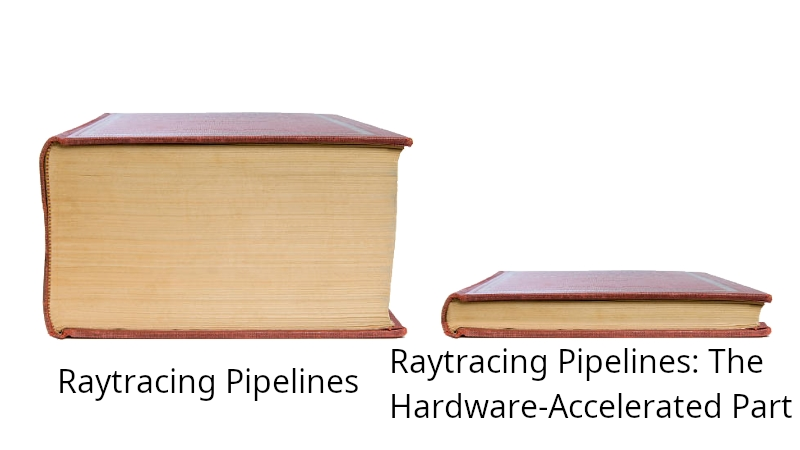
\includegraphics{graphics/booksmeme.png}
\end{slide}

\begin{slide}{Layout of a Raytracing pipeline - XDC 2022}
  \texttt{void main() \{ \\
  \hspace*{8pt}uint32\_t shader\_id = raygen\_sbt[0]; \\
  \hspace*{8pt}while (shader\_id != 0) \{ \\
  \hspace*{16pt}switch (shader\_id) \{ \\
  \hspace*{24pt}// paste all shader code in here \\
  \hspace*{16pt}\} \\
  \hspace*{8pt}\} \\
  \}} \\
 Problem: Raytracing pipelines can get \textbf{big} (2000+ shaders)
 \begin{itemize}
  \item Size of shaders caused stack overflows during passes that operated recursively on blocks
  \item Does not work well with pipeline libraries - have to copy shader code around and defer actual compilation
 \end{itemize}
\end{slide}

\begin{slide}{Layout of a Raytracing pipeline - XDC 2023}
 ``Monolithic'' mode:
 \begin{itemize}
  \item All shaders are fully inlined
  \item No shader call overhead, potential for constant propagation
  \item No recursion, no support for pipeline libraries
 \end{itemize}
  % epicer LaTeX programming,
  \texttt{void traceRay() // always inlined \{ \\
  \hspace*{8pt}// paste traversal shader \\
  \hspace*{8pt}if (hit) \\
  \hspace*{16pt}// paste closest-hit shader; \\
  \hspace*{8pt}else \\
  \hspace*{16pt}// paste miss shader \\
  \}} \\
  \texttt{void main() \{ \\
  \hspace*{8pt}// paste raygen shader \\
  \}} \\
\end{slide}

\begin{slide}{Layout of a Raytracing pipeline - XDC 2023}
 ``Separate Compilation'' mode:
 \begin{itemize}
  \item ``True'' shader calls - actual indirect jump
  \item Allows shaders from pipeline libraries to be compiled ahead of time
 \end{itemize}

 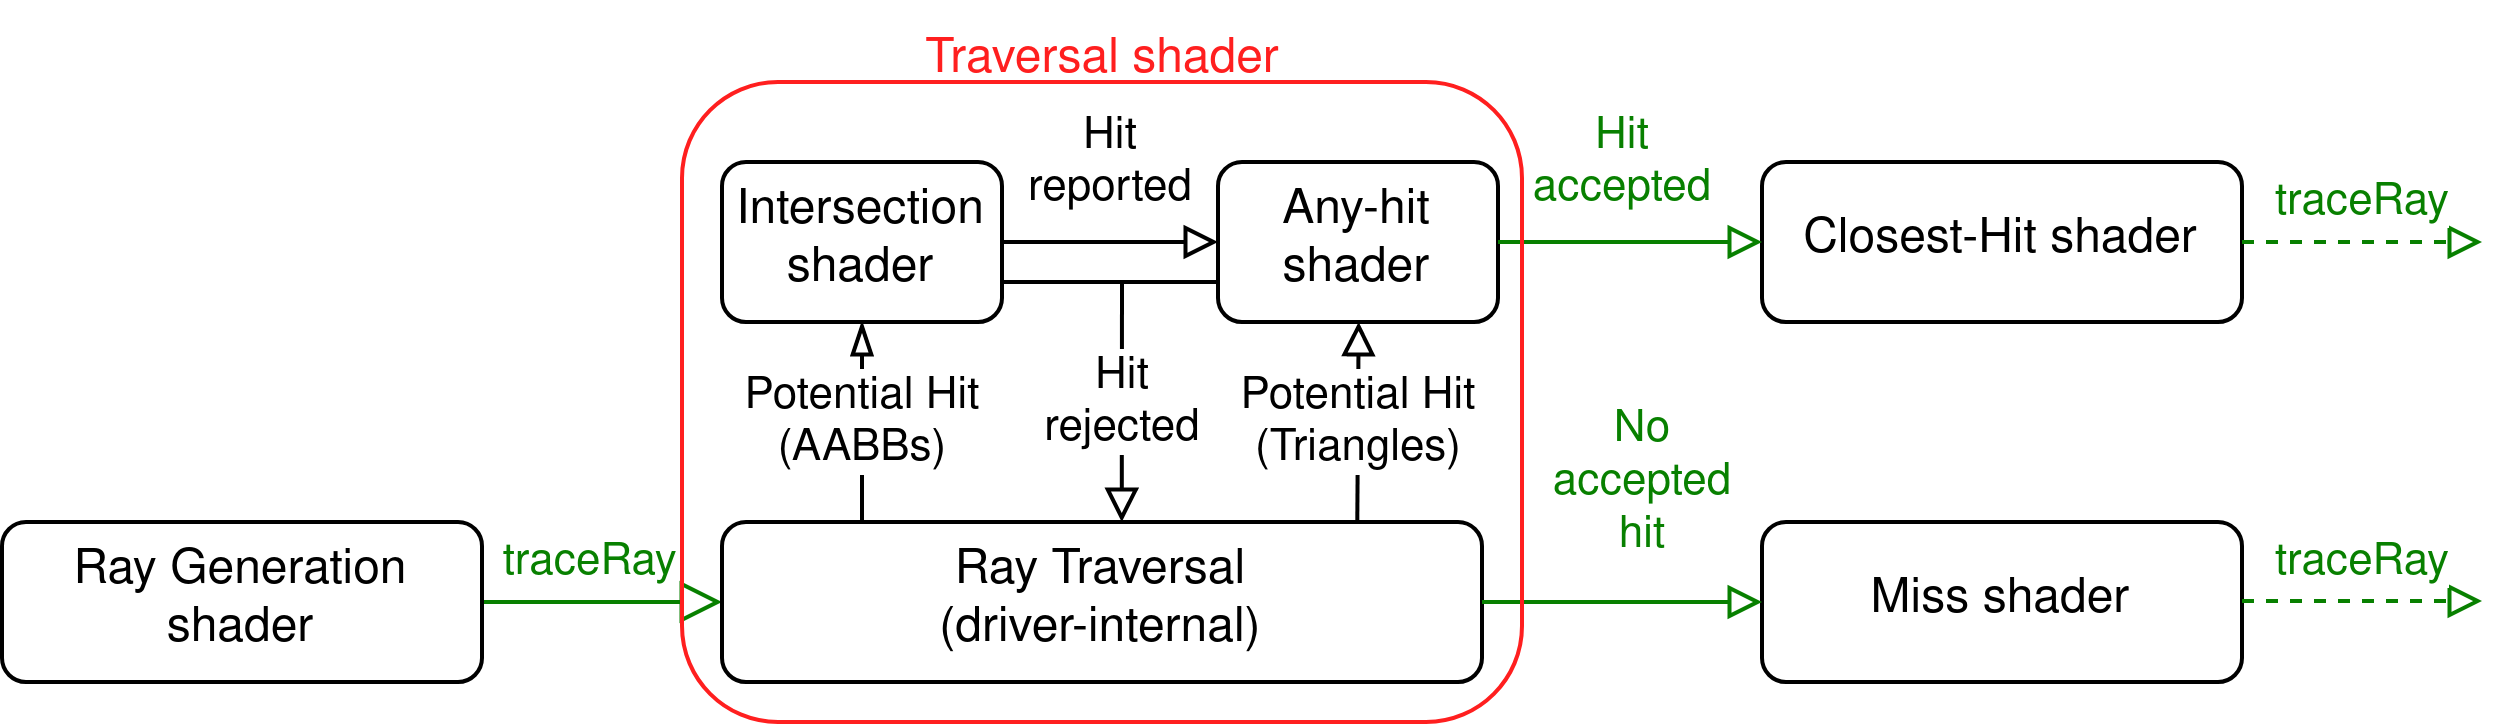
\includegraphics[width=1.0651\linewidth]{graphics/RTStages10.png}

\end{slide}

\begin{slide}{Layout of a Traversal Shader}
  \vspace*{-2pt} % sad hack, otherwise it doesn't fit :(
                 % nobody will notice
  % epic LaTeX programming
  \texttt{void main() \{ \\
  \hspace*{8pt}while (!traversal\_complete) \{ \\
  \hspace*{16pt}uint32\_t node\_pointer = get\_next\_node(); \\
  \hspace*{16pt}intersection\_result result = image\_bvh\_intersect\_ray(node\_pointer); \\
  \hspace*{16pt}if (result.hit) \{ \\
  \hspace*{24pt}// paste any-hit/intersection shaders here \\
  \hspace*{24pt}if (!hit\_accepted) \\
  \hspace*{32pt}continue; \\
  \hspace*{16pt}\} \\
  \hspace*{8pt}\} \\
  \hspace*{8pt}if (hit) \\
  \hspace*{16pt}call\_closest\_hit(); \\
  \hspace*{8pt}else \\
  \hspace*{16pt}call\_miss(); \\
  \}} \\
\end{slide}

\begin{slide}{Why not separately-compile the traversal shader?}
 \begin{itemize}
  \item Ray Traversal has lots of live state
  \item Any-Hit/Intersection shaders are relatively small yet called often
  \item High shader call overhead, negatively impacts performance
 \end{itemize}
\end{slide}

\begin{slide}{Implementing ``True'' Shader Calls}
 \begin{itemize}
  \item Jump execution to arbitrary addresses stored in SBT
  \item Each invocation in a wavefront may have a different address
  \item Only one program counter per wavefront
  \item Naive solution: Choose program counter of first valid invocation
  \item Guard shader invocations to prevent invocations from executing wrong shaders
  \item Problem: Reconvergent shader calls become inefficient!
 \end{itemize}
 \pause
 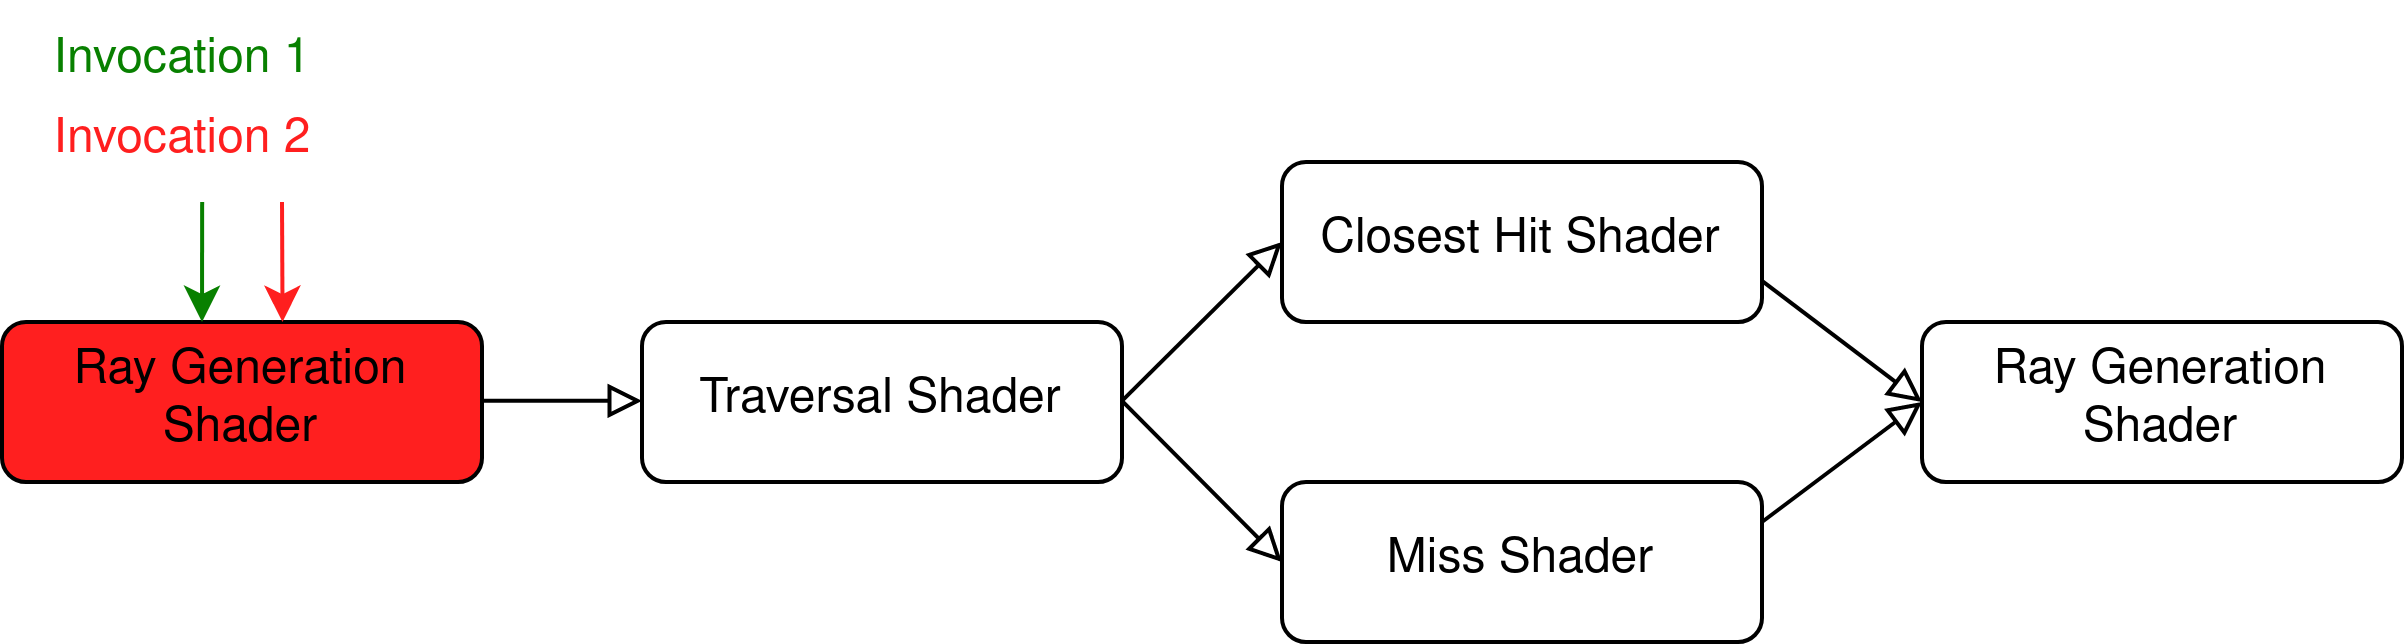
\includegraphics[width=\textwidth]{graphics/RTStages2-1.png}
\end{slide}

\begin{slide}{Implementing ``True'' Shader Calls}
 \begin{itemize}
  \item Jump execution to arbitrary addresses stored in SBT
  \item Each invocation in a wavefront may have a different address
  \item Only one program counter per wavefront
  \item Naive solution: Choose program counter of first valid invocation
  \item Guard shader invocations to prevent invocations from executing wrong shaders
  \item Problem: Reconvergent shader calls become inefficient!
 \end{itemize}
 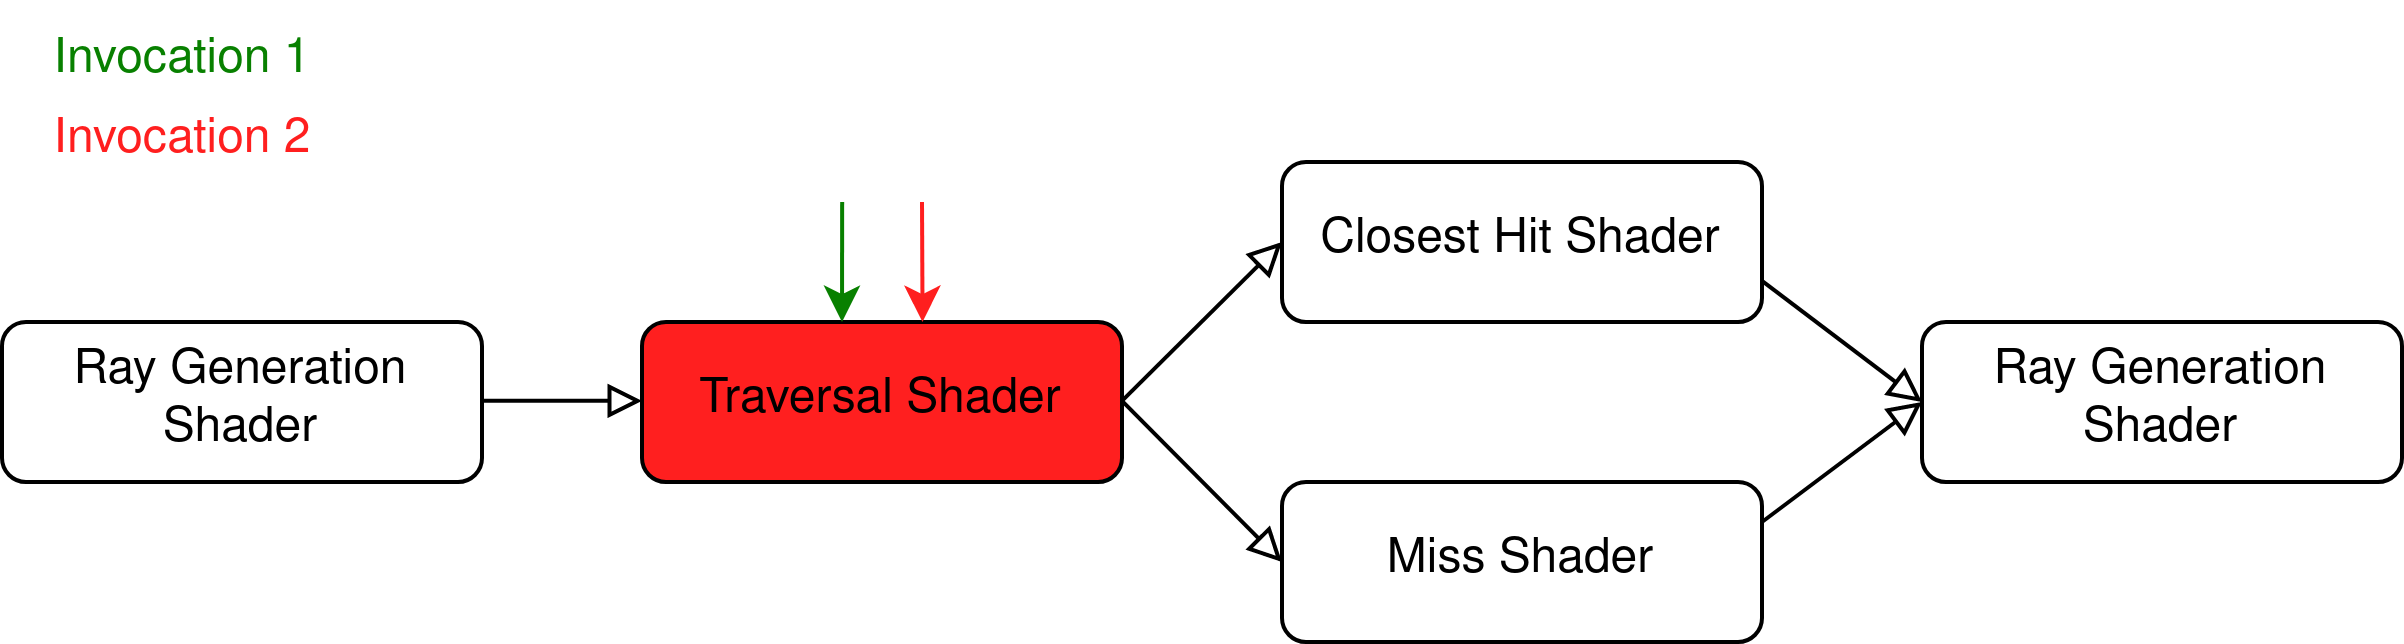
\includegraphics[width=\textwidth]{graphics/RTStages2-2.png}
\end{slide}

\begin{slide}{Implementing ``True'' Shader Calls}
 \begin{itemize}
  \item Jump execution to arbitrary addresses stored in SBT
  \item Each invocation in a wavefront may have a different address
  \item Only one program counter per wavefront
  \item Naive solution: Choose program counter of first valid invocation
  \item Guard shader invocations to prevent invocations from executing wrong shaders
  \item Problem: Reconvergent shader calls become inefficient!
 \end{itemize}
 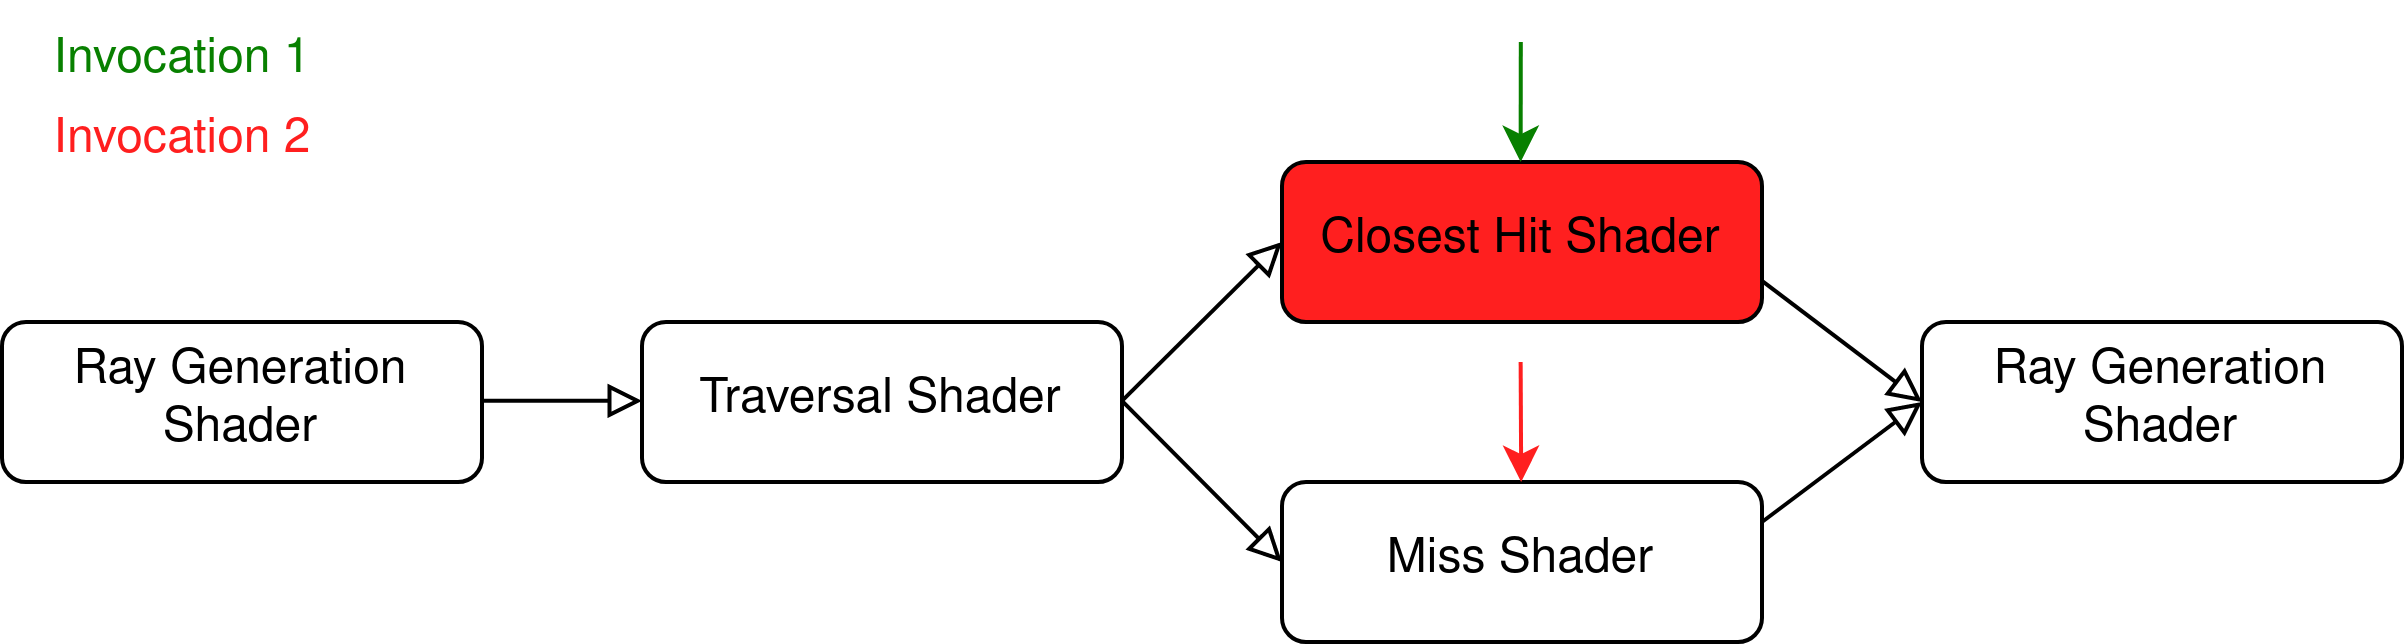
\includegraphics[width=\textwidth]{graphics/RTStages2-3.png}
\end{slide}

\begin{slide}{Implementing ``True'' Shader Calls}
 \begin{itemize}
  \item Jump execution to arbitrary addresses stored in SBT
  \item Each invocation in a wavefront may have a different address
  \item Only one program counter per wavefront
  \item Naive solution: Choose program counter of first valid invocation
  \item Guard shader invocations to prevent invocations from executing wrong shaders
  \item Problem: Reconvergent shader calls become inefficient!
 \end{itemize}
 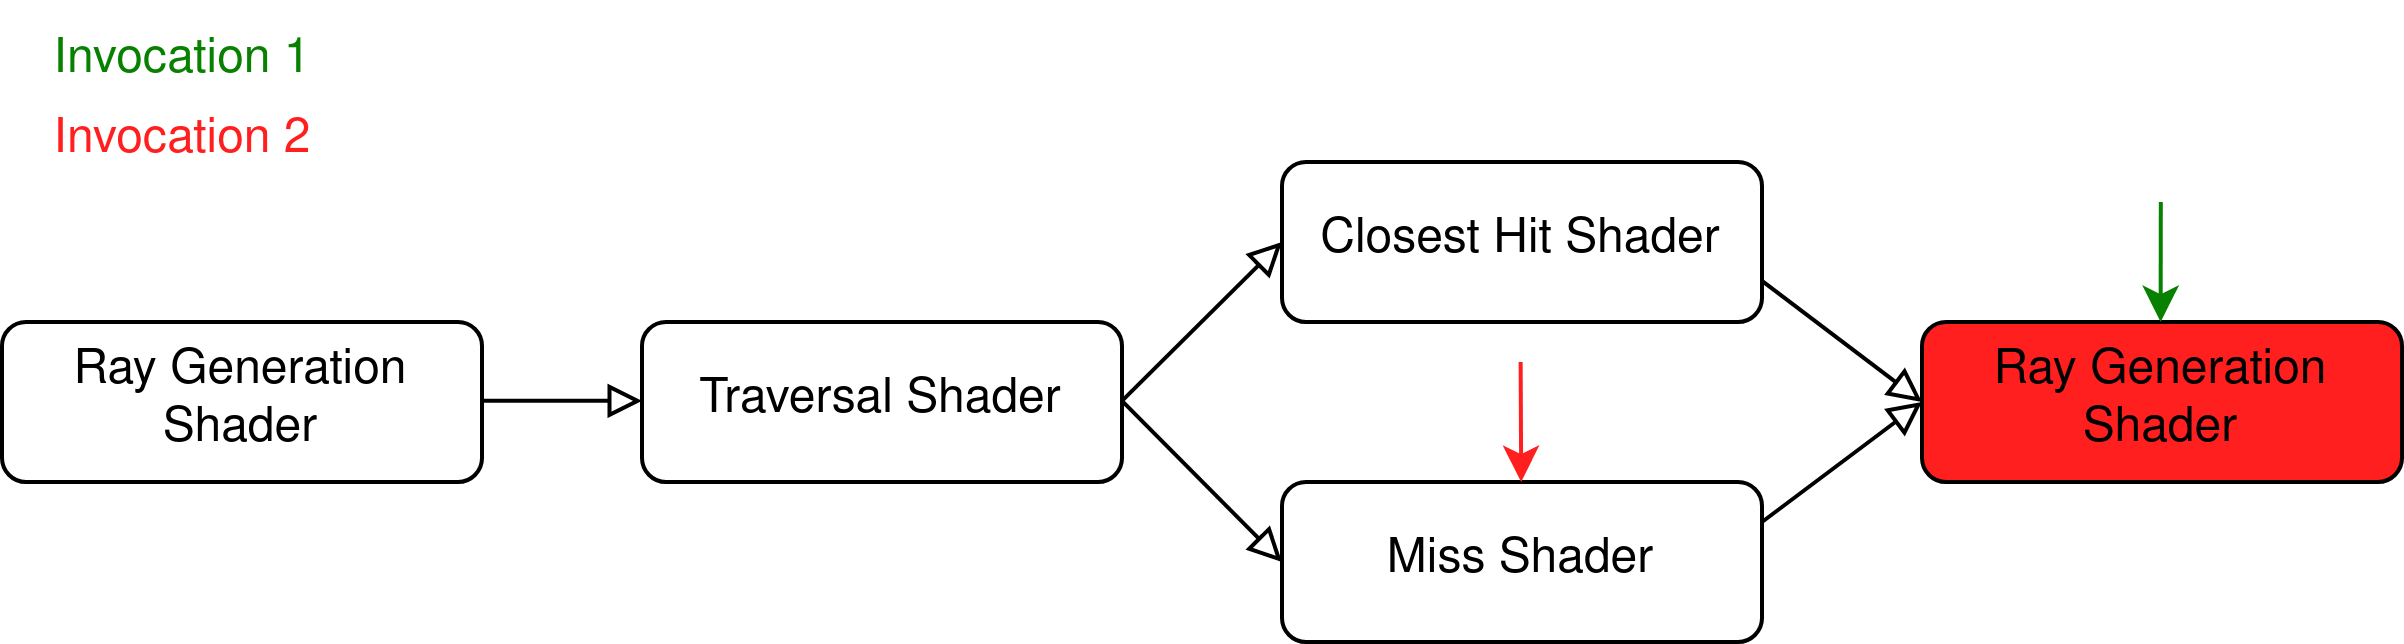
\includegraphics[width=\textwidth]{graphics/RTStages2-4.png}
\end{slide}

\begin{slide}{Implementing ``True'' Shader Calls}
 \begin{itemize}
  \item Jump execution to arbitrary addresses stored in SBT
  \item Each invocation in a wavefront may have a different address
  \item Only one program counter per wavefront
  \item Naive solution: Choose program counter of first valid invocation
  \item Guard shader invocations to prevent invocations from executing wrong shaders
  \item Problem: Reconvergent shader calls become inefficient!
 \end{itemize}
 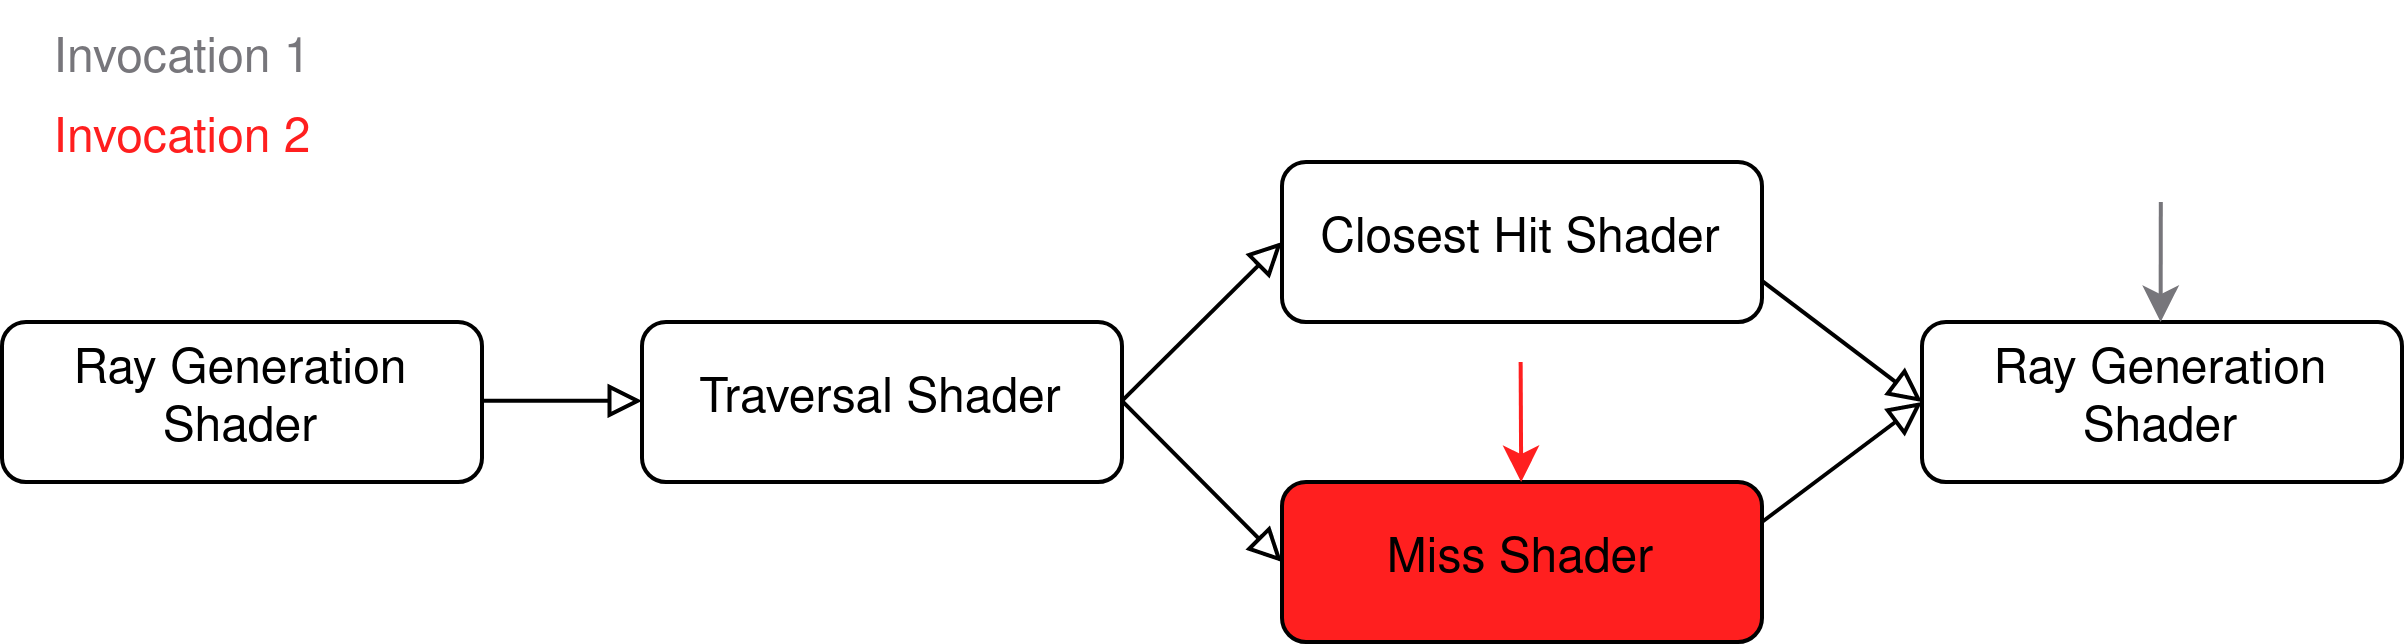
\includegraphics[width=\textwidth]{graphics/RTStages2-5.png}
\end{slide}

\begin{slide}{Implementing ``True'' Shader Calls}
 \begin{itemize}
  \item Jump execution to arbitrary addresses stored in SBT
  \item Each invocation in a wavefront may have a different address
  \item Only one program counter per wavefront
  \item Naive solution: Choose program counter of first valid invocation
  \item Guard shader invocations to prevent invocations from executing wrong shaders
  \item Problem: Reconvergent shader calls become inefficient!
 \end{itemize}
 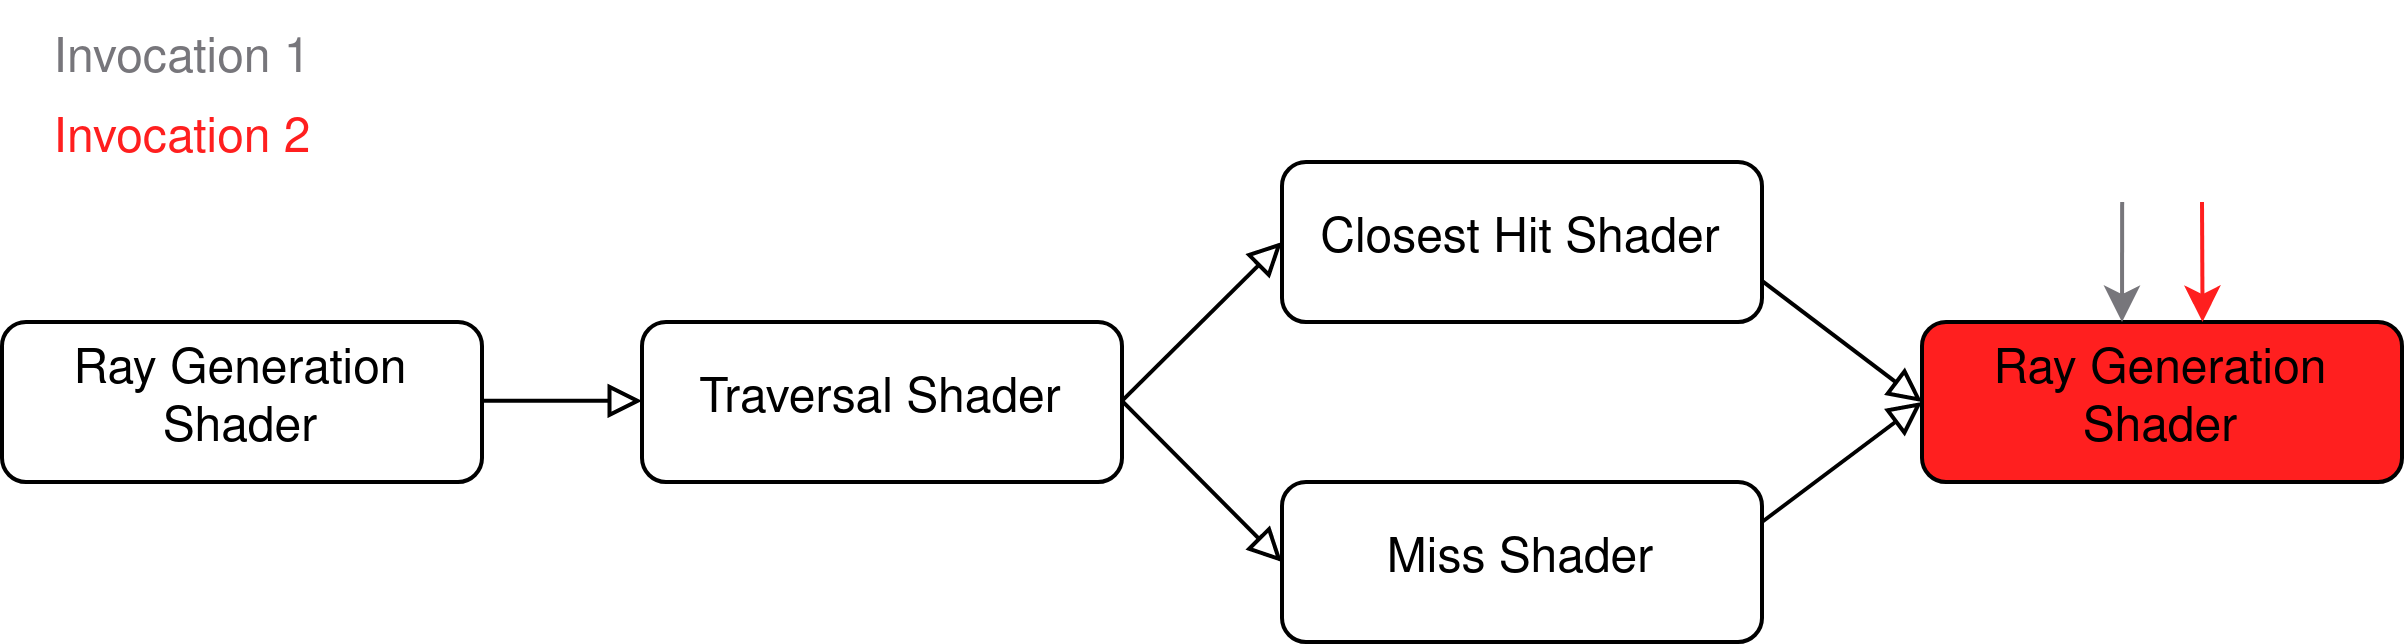
\includegraphics[width=\textwidth]{graphics/RTStages2-6.png}
\end{slide}

\begin{slide}{Implementing ``True'' Shader Calls}
 \begin{itemize}
  \item Solution: Select shader based on type
  \item Certain shader types will always be preferred over others
  \item Prefer Hit/Miss over Traversal shaders
  \item Execute Raygen only when no other shaders are available
  \item Shader type is packed into the 4 LSBs of the shader's address
 \end{itemize}
 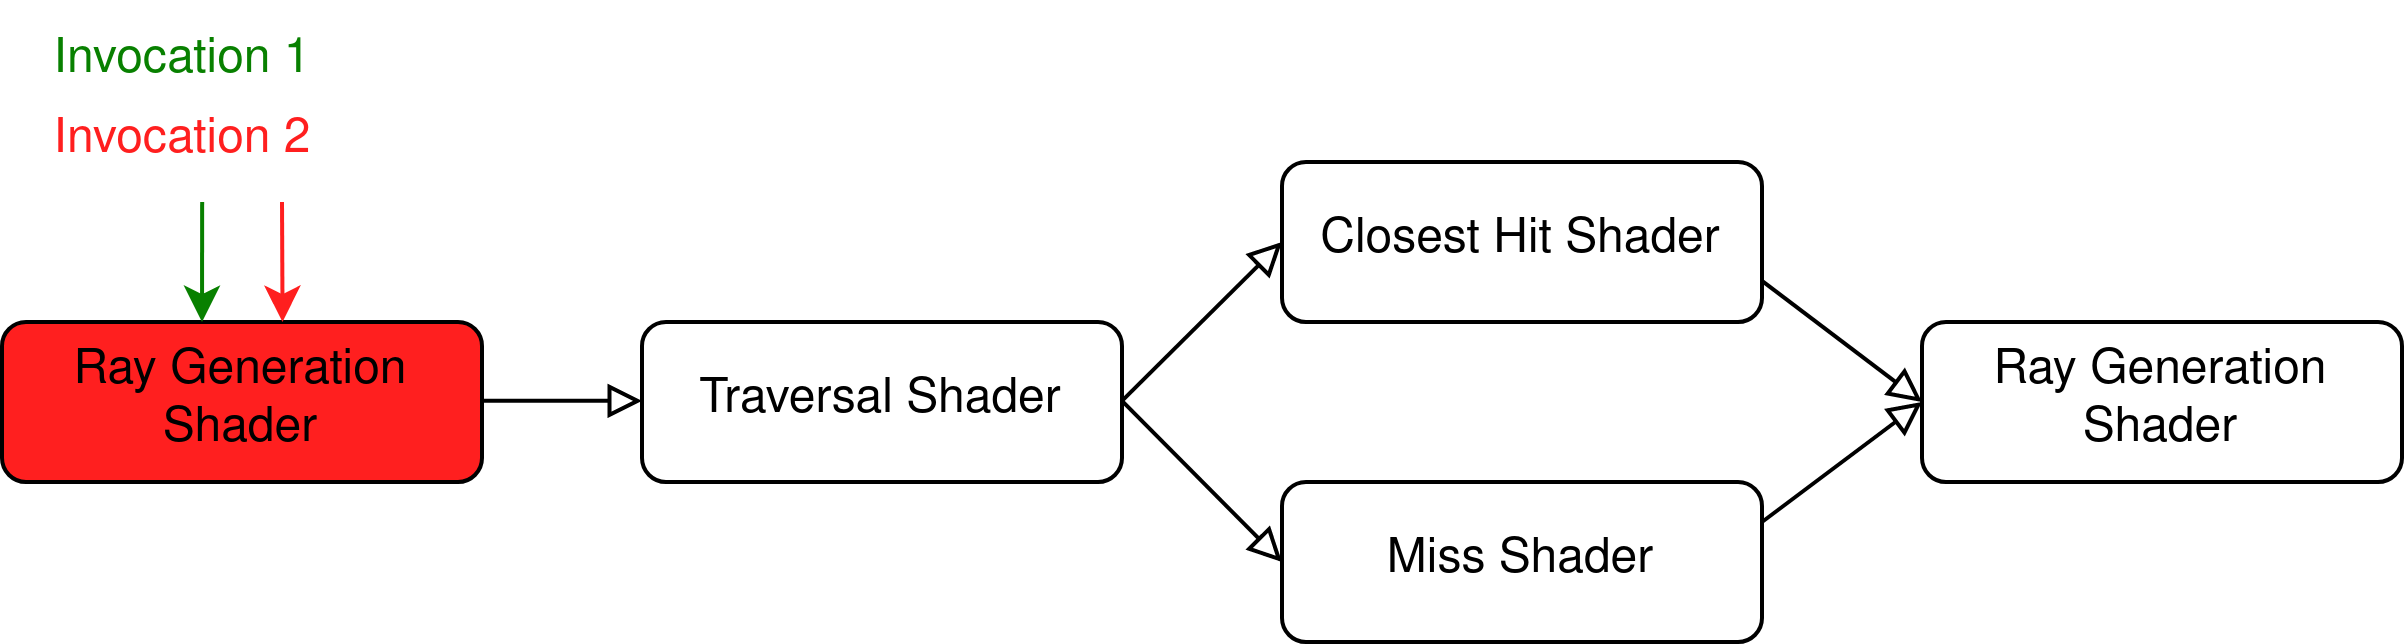
\includegraphics[width=\textwidth]{graphics/RTStages2-1.png}
\end{slide}

\begin{slide}{Implementing ``True'' Shader Calls}
 \begin{itemize}
  \item Solution: Select shader based on type
  \item Certain shader types will always be preferred over others
  \item Prefer Hit/Miss over Traversal shaders
  \item Execute Raygen only when no other shaders are available
  \item Shader type is packed into the 4 LSBs of the shader's address
 \end{itemize}
 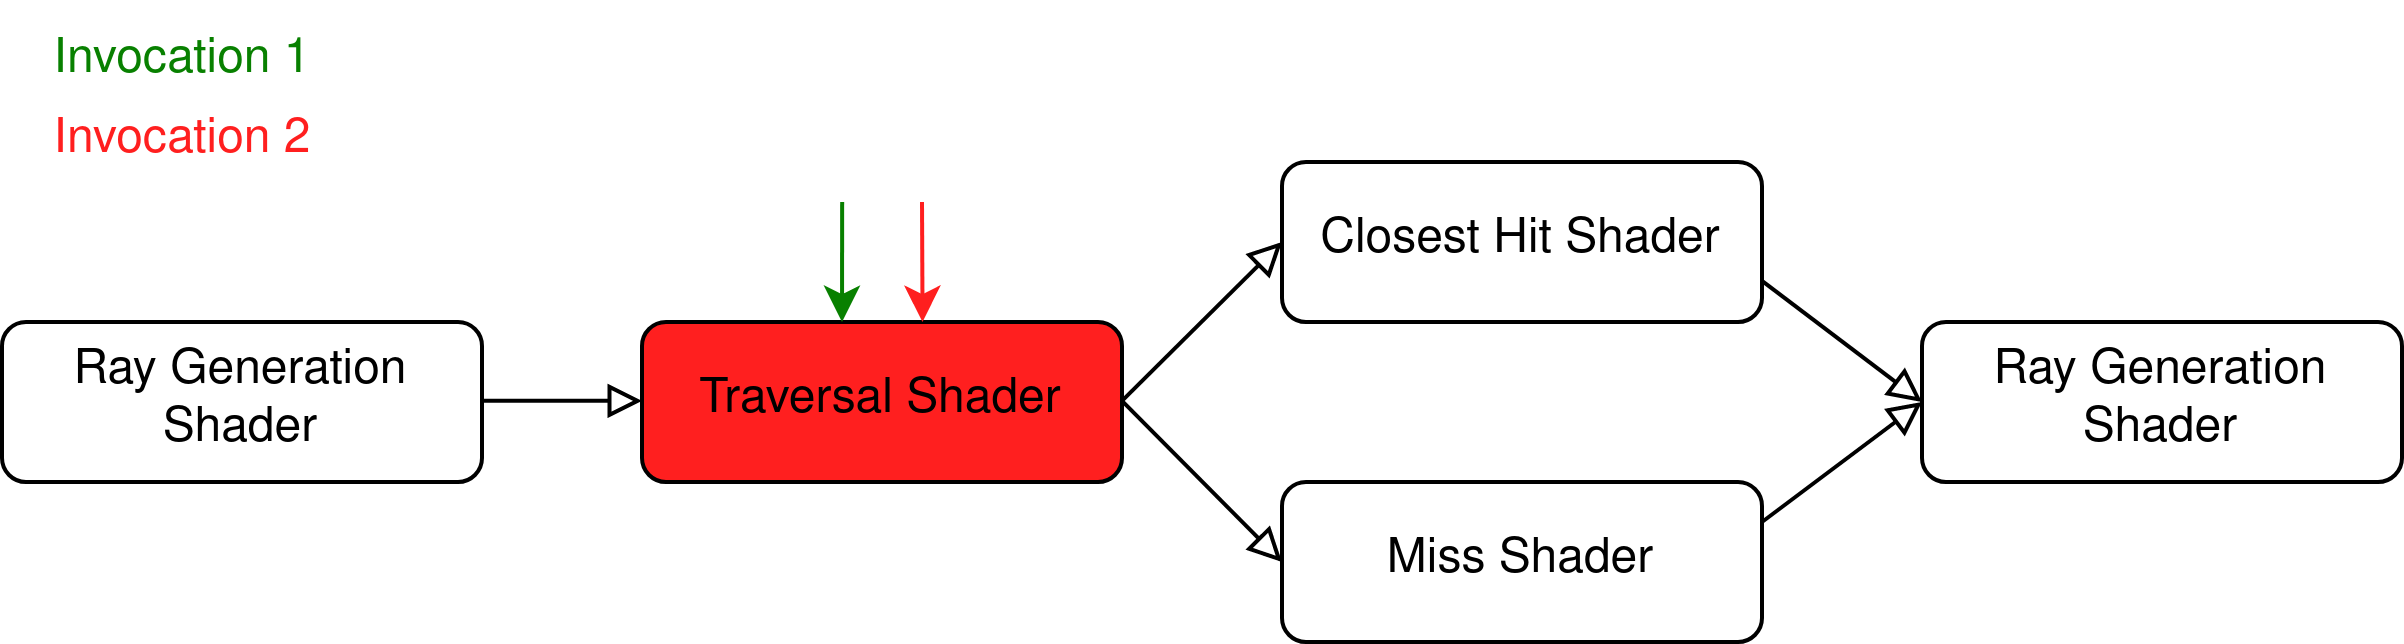
\includegraphics[width=\textwidth]{graphics/RTStages2-2.png}
\end{slide}

\begin{slide}{Implementing ``True'' Shader Calls}
 \begin{itemize}
  \item Solution: Select shader based on type
  \item Certain shader types will always be preferred over others
  \item Prefer Hit/Miss over Traversal shaders
  \item Execute Raygen only when no other shaders are available
  \item Shader type is packed into the 4 LSBs of the shader's address
 \end{itemize}
 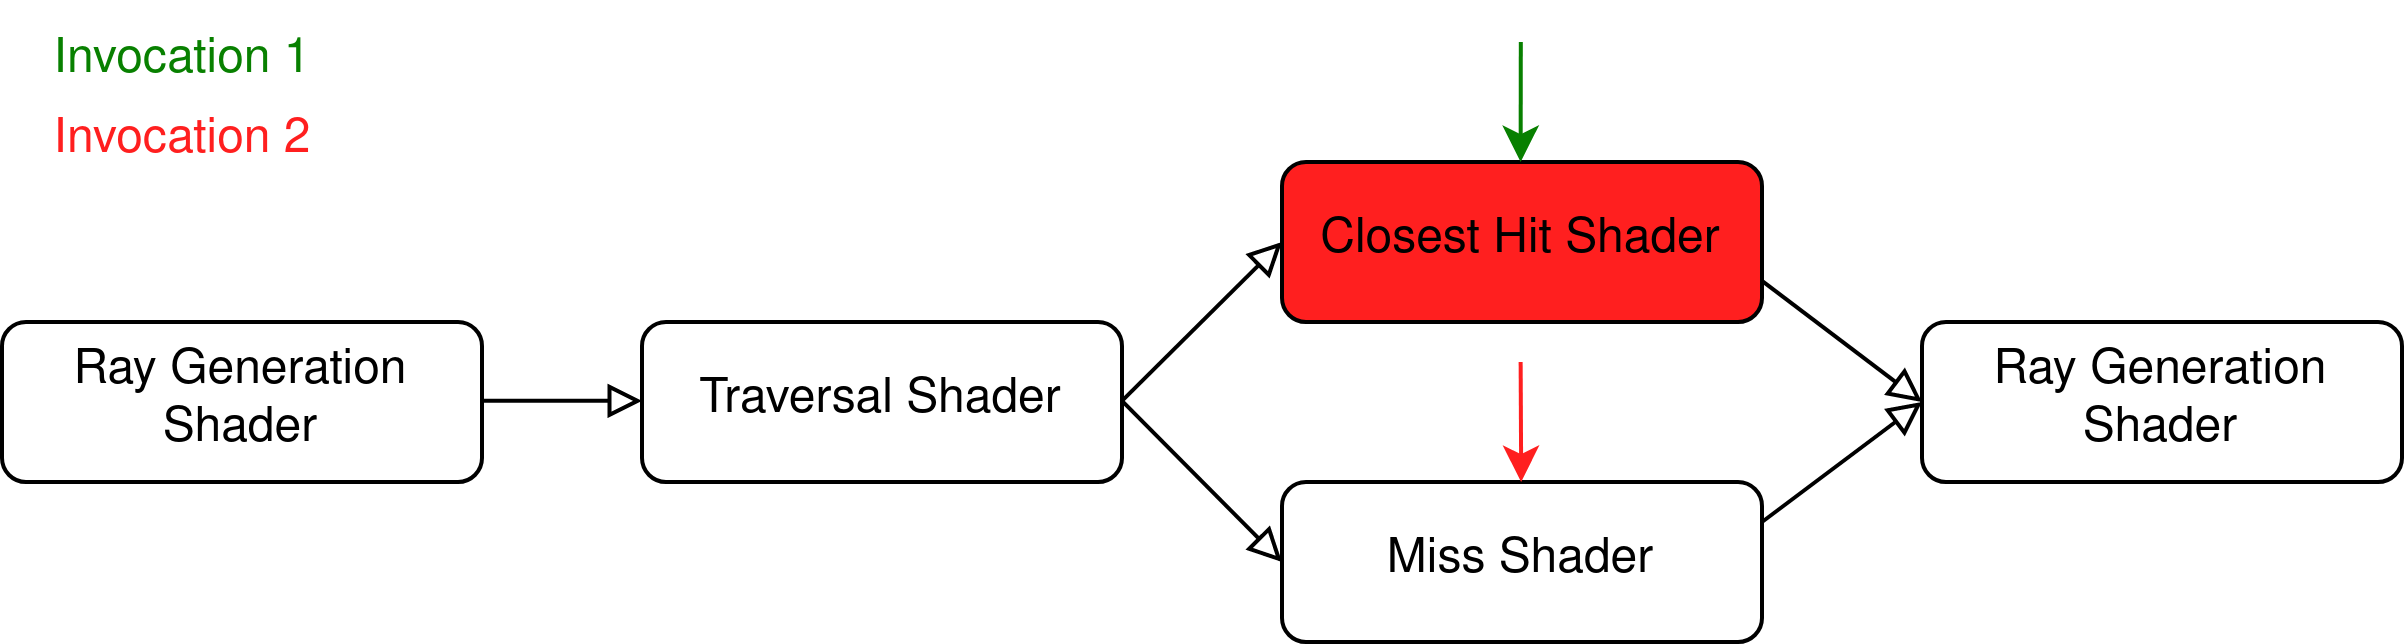
\includegraphics[width=\textwidth]{graphics/RTStages2-3.png}
\end{slide}

\begin{slide}{Implementing ``True'' Shader Calls}
 \begin{itemize}
  \item Solution: Select shader based on type
  \item Certain shader types will always be preferred over others
  \item Prefer Hit/Miss over Traversal shaders
  \item Execute Raygen only when no other shaders are available
  \item Shader type is packed into the 4 LSBs of the shader's address
 \end{itemize}
 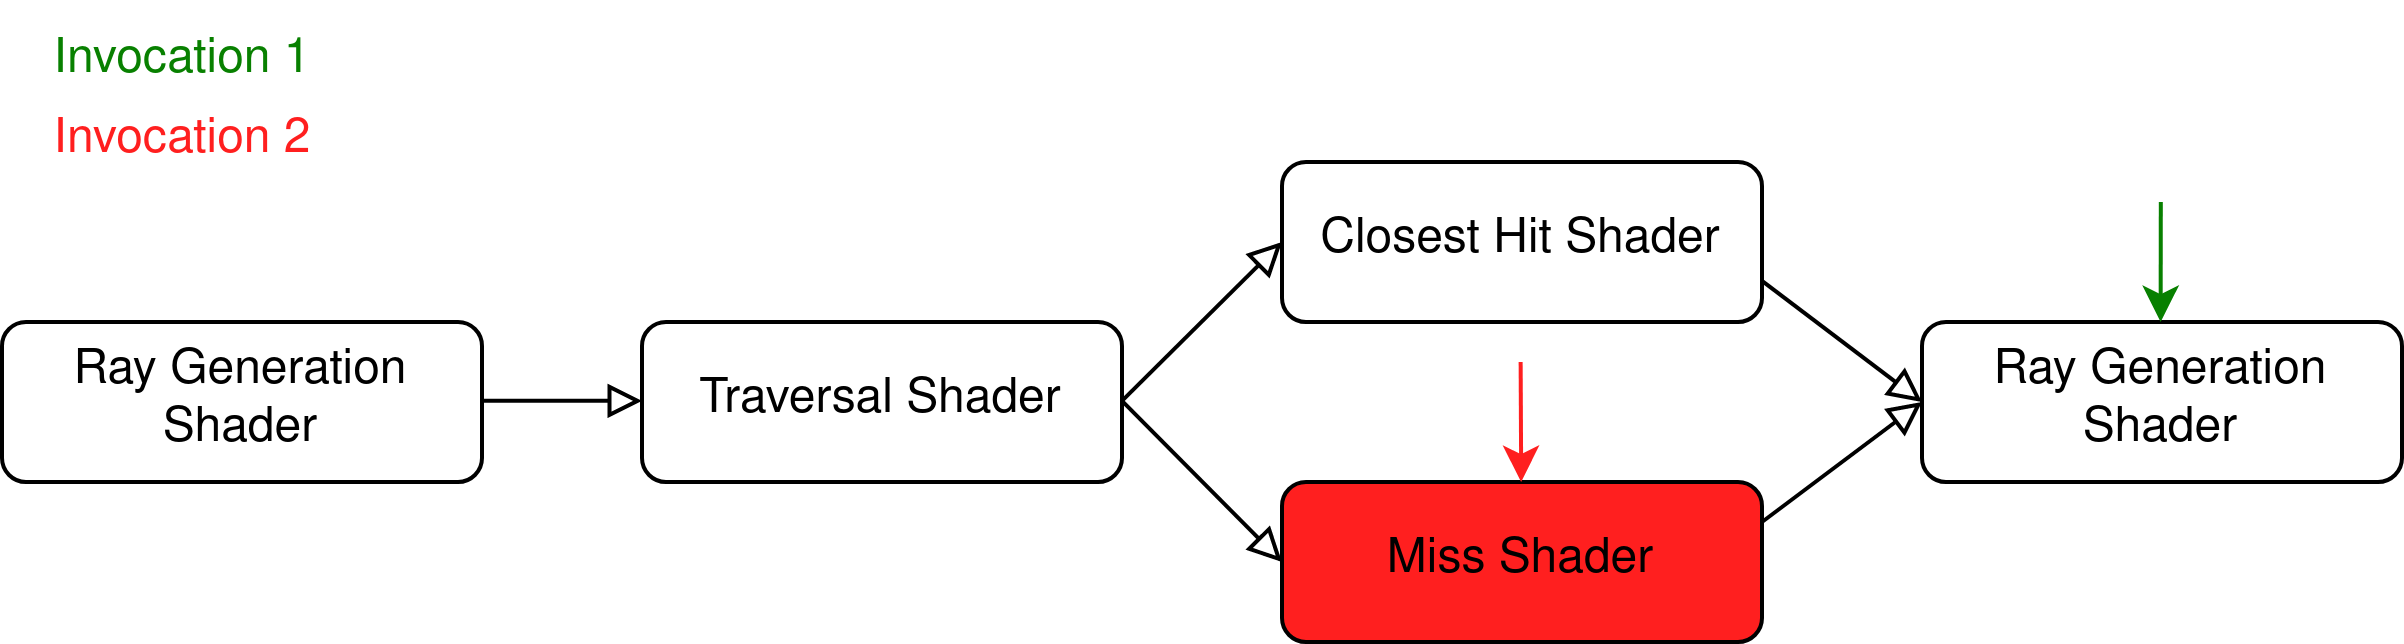
\includegraphics[width=\textwidth]{graphics/RTStages2-7.png}
\end{slide}

\begin{slide}{Implementing ``True'' Shader Calls}
 \begin{itemize}
  \item Solution: Select shader based on type
  \item Certain shader types will always be preferred over others
  \item Prefer Hit/Miss over Traversal shaders
  \item Execute Raygen only when no other shaders are available
  \item Shader type is packed into the 4 LSBs of the shader's address
 \end{itemize}
 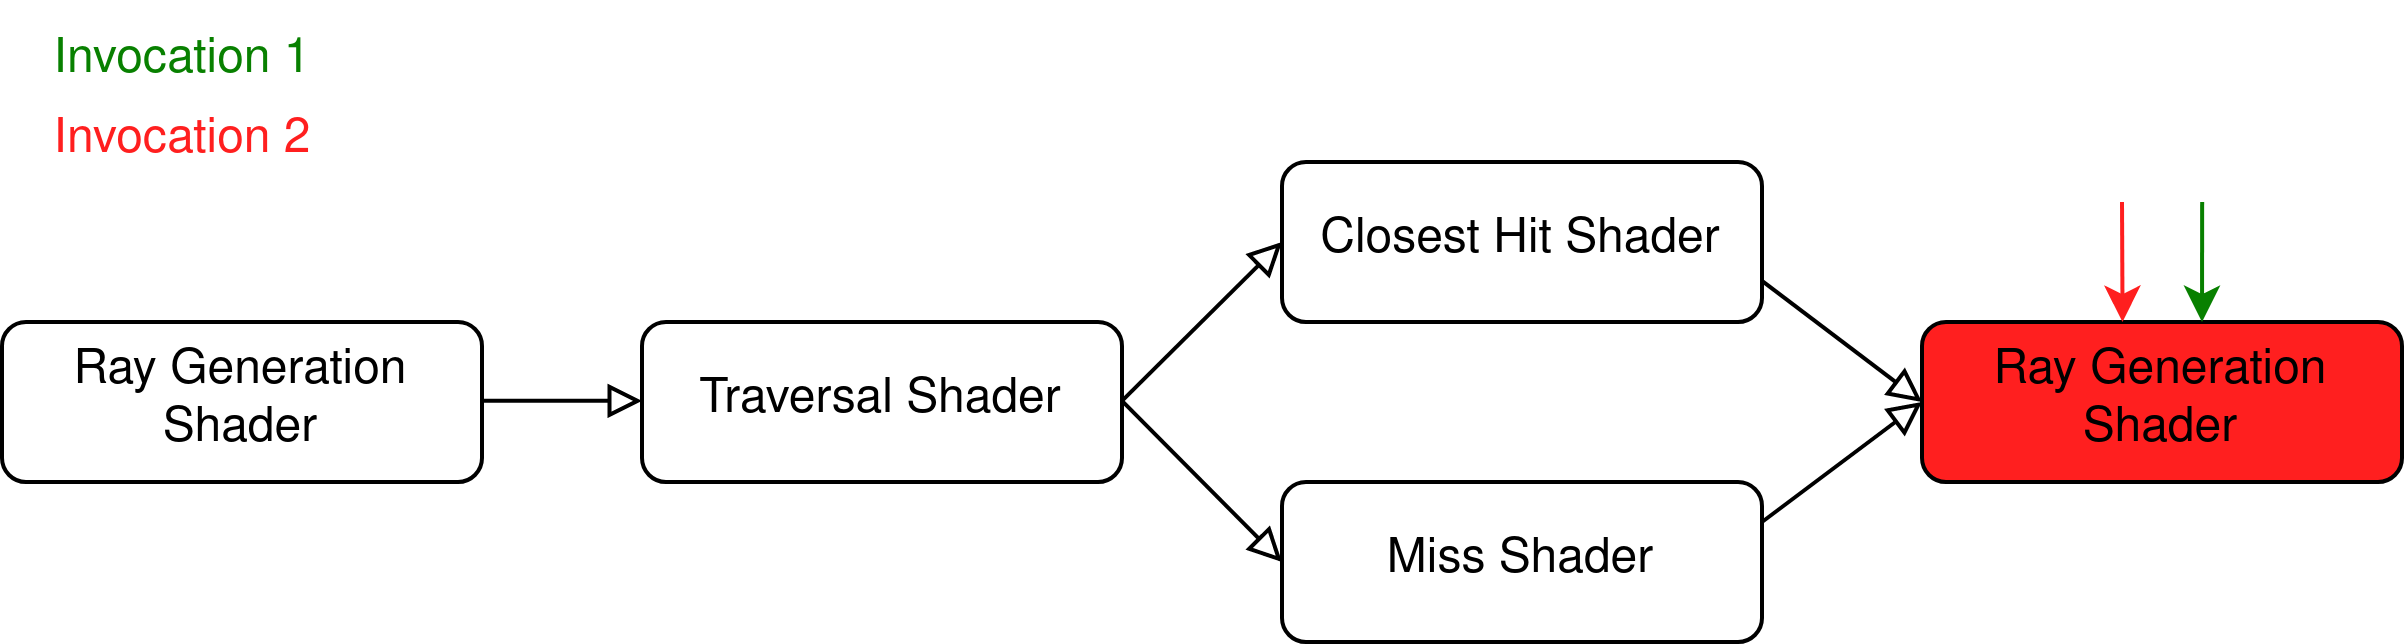
\includegraphics[width=\textwidth]{graphics/RTStages2-8.png}
\end{slide}


\section{Case Studies: Why Some Games Were Broken}

\chapterIntroConfig
\begin{slide}{Case Studies: Why Some Games Were Broken}
\end{slide}
\defaultConfig

\subsection{DOOM Eternal}
\subsection{Cyberpunk 2077}
\subsection{Nearly All Other D3D12 Games}

\section{What's To Come}

\chapterIntroConfig
\begin{slide}{What's To Come}
\end{slide}
\defaultConfig

\subsection{Where We Are}
\subsection{Where We're Going}

\end{document}

